\documentclass[letterpaper]{article}
\usepackage{amsmath}
\usepackage{tikz}
\usepackage{epigraph}
\usepackage{lipsum}
\usepackage{hyperref}
\usepackage{tocloft}
\usepackage{graphicx}
\usepackage{float}

\usepackage{setspace, amsmath}

\usepackage[centering,includeheadfoot,margin=2cm]{geometry}
\usepackage{xcolor}
\usepackage{calc,blindtext}

\renewcommand\epigraphflush{flushright}
\renewcommand\epigraphsize{\normalsize}
\setlength\epigraphwidth{0.6\textwidth}

\definecolor{titlepagecolor}{cmyk}{1,.60,0,.40}

\DeclareFixedFont{\titlefont}{T1}{ppl}{b}{it}{1.0in}

\makeatletter
\def\printauthor{%
    {\large \@author}}
\makeatother
\author{%
    Nico Taljaard \\
    10153285 \vspace{20pt} \\
    Gerhard Smit \\
    12282945 \vspace{20pt} \\
    Martin Schoeman \\
    10651994 \\
}

% The following code is borrowed from: http://tex.stackexchange.com/a/86310/10898

\newcommand\titlepagedecoration{%
	\begin{tikzpicture}[remember picture,overlay,shorten >= -10pt]
	
		\coordinate (aux1) at ([yshift=-15pt]current page.north east);
		\coordinate (aux2) at ([yshift=-410pt]current page.north east);
		\coordinate (aux3) at ([xshift=-4.5cm]current page.north east);
		\coordinate (aux4) at ([yshift=-150pt]current page.north east);
		
		\begin{scope}[titlepagecolor!40,line width=12pt,rounded corners=12pt]
			\draw
			  (aux1) -- coordinate (a)
			  ++(225:5) --
			  ++(-45:5.1) coordinate (b);
			\draw[shorten <= -10pt]
			  (aux3) --
			  (a) --
			  (aux1);
			\draw[opacity=0.6,titlepagecolor,shorten <= -10pt]
			  (b) --
			  ++(225:2.2) --
			  ++(-45:2.2);
		\end{scope}
			\draw[titlepagecolor,line width=8pt,rounded corners=8pt,shorten <= -10pt]
			  (aux4) --
			  ++(225:0.8) --
			  ++(-45:0.8);
		\begin{scope}[titlepagecolor!70,line width=6pt,rounded corners=8pt]
			\draw[shorten <= -10pt]
			  (aux2) --
			  ++(225:3) coordinate[pos=0.45] (c) --
			  ++(-45:3.1);
			\draw
			  (aux2) --
			  (c) --
			  ++(135:2.5) --
			  ++(45:2.5) --
			  ++(-45:2.5) coordinate[pos=0.3] (d);   
			\draw 
			  (d) -- +(45:1);
		\end{scope}
	\end{tikzpicture}
}

\begin{document}

\begin{titlepage}

\noindent
\titlefont Laminin \par
\epigraph{ XGame - Derivco \\ Corspe Slasher \\ Functional requirements and application design}%
{\textit{ 01/08/2014 }\\ \textsc{ }}
\null\vfill
\vspace*{4cm}
\noindent
\hfill
\begin{minipage}{0.35\linewidth}
    \begin{flushright}
        \printauthor
    \end{flushright}
\end{minipage}
%
\begin{minipage}{0.02\linewidth}
    \rule{1pt}{125pt}
\end{minipage}
\titlepagedecoration
\end{titlepage}

% % % % % % % % % % % % % % %
% 							%
%	Remainder of document	%
% 							%
% % % % % % % % % % % % % % % 

	\newpage
		{\LARGE \bf Change Log}\\[2em]
		
		\begin{tabbing}
			\hspace*{2.5cm}\=\hspace*{2.5cm}\=\hspace*{8cm}\=\hspace*{3cm} \kill
			28/07/2014	\> Version 1.0	\> Document Created 							\> Nico Taljaard \\
			29/07/2014	\> Version 1.0	\> Added game class diagram						\> Nico Taljaard \\
			29/07/2014	\> Version 1.0	\> Added game use case diagram					\> Nico Taljaard \\
			30/07/2014	\> Version 1.1	\> Change document structure					\> Nico Taljaard \\
			30/07/2014	\> Version 1.1	\> Added introduction							\> Nico Taljaard \\
			30/07/2014  \> Version 1.1  \> Added Server use case diagram				\> Martin Schoeman\\
			30/07/2014  \> Version 1.1  \> Added OAuth use case diagram					\> Martin Schoeman\\
			30/07/2014  \> Version 1.1  \> Added server class diagram					\> Martin Schoeman\\
			31/07/2014  \> Version 1.1  \> Added code documentation						\> Nico Taljaard\\
			31/07/2014  \> Version 1.1  \> Added mob state diagram						\> Nico Taljaard\\
			31/07/2014  \> Version 1.1  \> Added server state diagram					\> Martin Schoeman\\
			31/07/2014  \> Version 1.1  \> Added user-interface case diagrams			\> Gerhard Smit\\
			01/08/2014  \> Version 1.1  \> Added user-interface class diagrams			\> Gerhard Smit\\
			01/08/2014  \> Version 1.1  \> Added services contracts for user-interface 			\> Gerhard Smit\\
			01/08/2014  \> Version 1.1  \> Finished off services contracts and added \> \\
			\> \>  state diagram for User-Interface \> Gerhard Smit\\
			01/08/2014  \> Version 1.1  \> Added GUI screen shots						\> Gerhard Smit\\
			01/08/2014  \> Version 1.1  \> Added database ERD diagram.						\> Martin Schoeman\\
			01/08/2014  \> Version 1.1  \> Document finalization.						\> Nico Taljaard\\
		\end{tabbing}
		
	\newpage
		\renewcommand\contentsname{TABLE OF CONTENTS}
		\newcommand\contentsnameLC{\colorbox{blue}{\makebox[\textwidth-2\fboxsep][l]{\bfseries\color{white} Table of Contents}}}
		
		\renewcommand{\cftdot}{}
		\hypersetup{linktocpage}
		\tableofcontents
		
		\begin{flushleft}
			\LARGE\href{https://github.com/njTaljaard/Laminin_CorpseSlasher/}{Git repository: Laminin - Corpse Slasher}
		\end{flushleft}
		
	\newpage
		
		\section*{\colorbox{blue}{\makebox[\textwidth-2\fboxsep][l]{\bfseries\color{white} Introduction }}} \addcontentsline{toc}{section}{Introduction}
		\vspace{0.1in}
			
			Derivco as a stakeholder requires a game developed with open source software. Users should be able to create a custom account for the game or log into the game through their Facebook or Google accounts. A player should be able to walk around in a scene filled with computer controlled enemies. Upon the detection of a player the mob will attack it, the player should be able to fight back and kill the enemy or die. Users can change the graphical settings, display settings and sound settings of the game after they have logged into the game. A leader board should be accessible within the game which will rank users according to the points earned from killing mobs.
			
		\section*{\colorbox{blue}{\makebox[\textwidth-2\fboxsep][l]{\bfseries\color{white} Functional Requirements }}} \addcontentsline{toc}{section}{Functional Requirements}
		\vspace{0.1in}
		
			\subsection*{Required Functionality:}
			\addcontentsline{toc}{subsection}{Required Functionality}
			\vspace{0.1in}
			
				\subsubsection*{Game Diagrams:}
				\addcontentsline{toc}{subsubsection}{Game Diagrams}
				\vspace{0.2in}
				
					\begin{figure}[H]
					\centering
					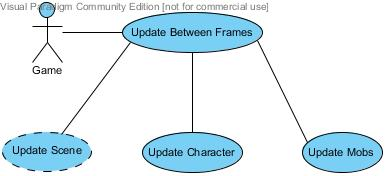
\includegraphics[width=140mm]{UML_Diagram/Use_Case/Game_Process.jpg}
					\caption{Update process between frames}
					\end{figure}
					
					\begin{figure}[H]
					\centering
					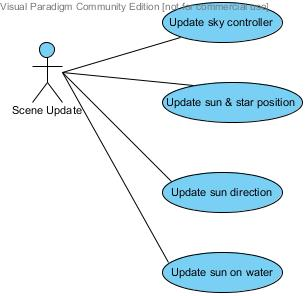
\includegraphics[width=140mm, height=100mm]{UML_Diagram/Use_Case/Update_Scene.jpg}
					\caption{Update of scene elements}
					\end{figure}
					
					\begin{figure}[H]
					\centering
					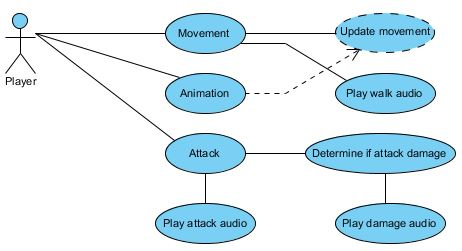
\includegraphics[width=140mm]{UML_Diagram/Use_Case/Player_Actions.jpg}
					\caption{Actions available to player}
					\end{figure}
					
					\begin{figure}[H]
					\centering
					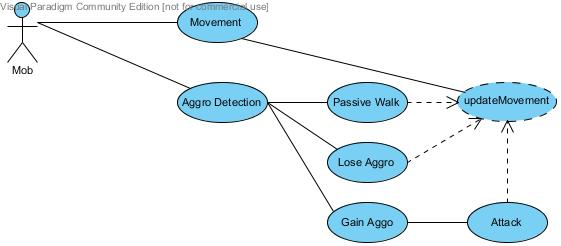
\includegraphics[width=140mm]{UML_Diagram/Use_Case/Mob_Actions.jpg}
					\caption{Actions available to mobs}
					\end{figure}
					
				\vspace{0.2in}
				\subsubsection*{User-interface Diagrams:}
				\addcontentsline{toc}{subsubsection}{User-interface Diagrams}
				\vspace{0.2in}
				
					\begin{figure}[H]
					\centering
					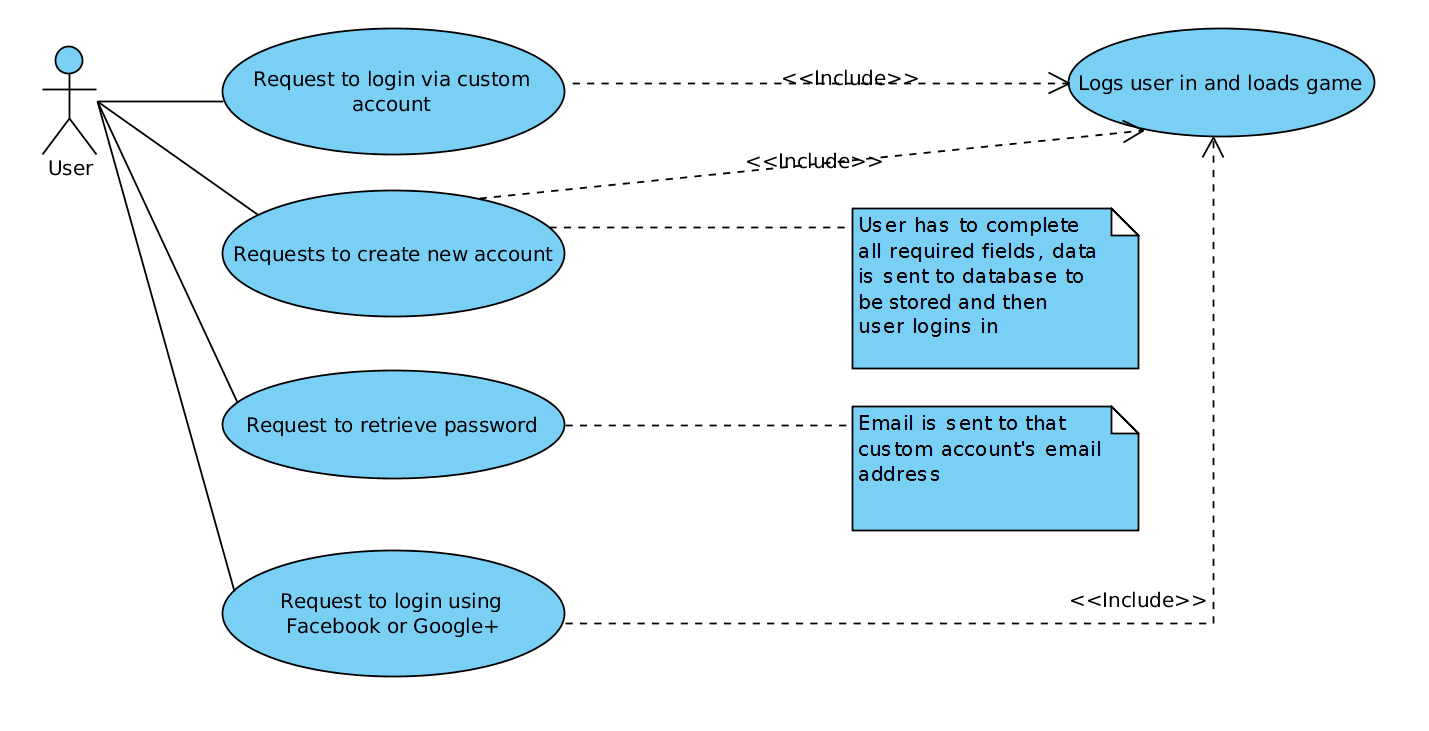
\includegraphics[width=140mm]{UML_Diagram/Use_Case/User_Login.jpg}
					\caption{User Login Screen}
					\end{figure}
				
					\begin{figure}[H]
					\centering
					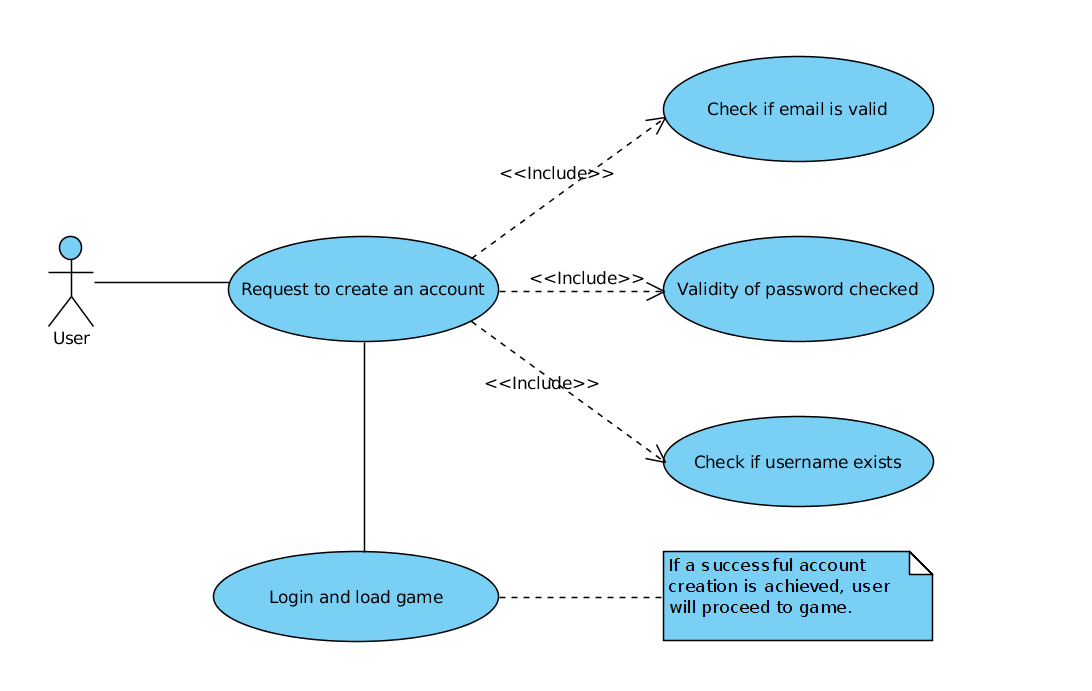
\includegraphics[width=140mm]{UML_Diagram/Use_Case/CreatAccount_UseCase.jpg}
					\caption{Create New Account Screen}
					\end{figure}
				
					\begin{figure}[H]
					\centering
					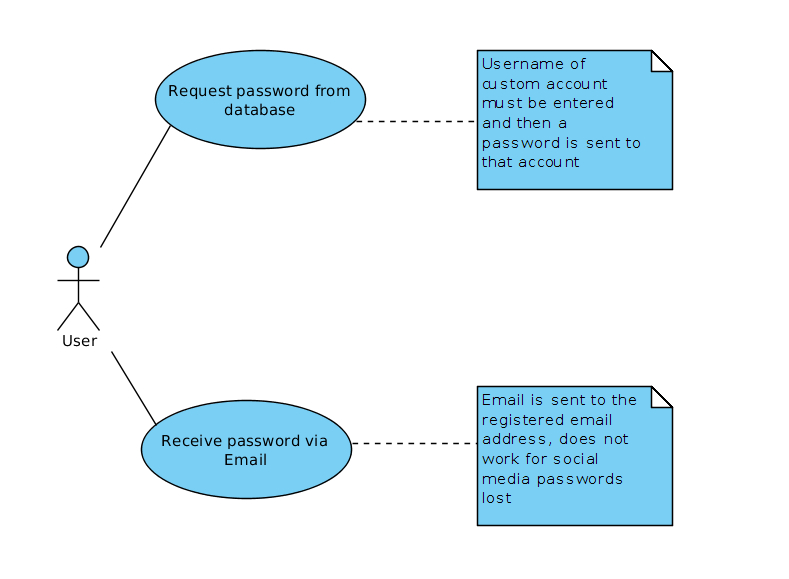
\includegraphics[width=140mm]{UML_Diagram/Use_Case/RetrievePassword_UseCase.jpg}
					\caption{Retrieve Password Screen}
					\end{figure}
				
					\begin{figure}[H]
					\centering
					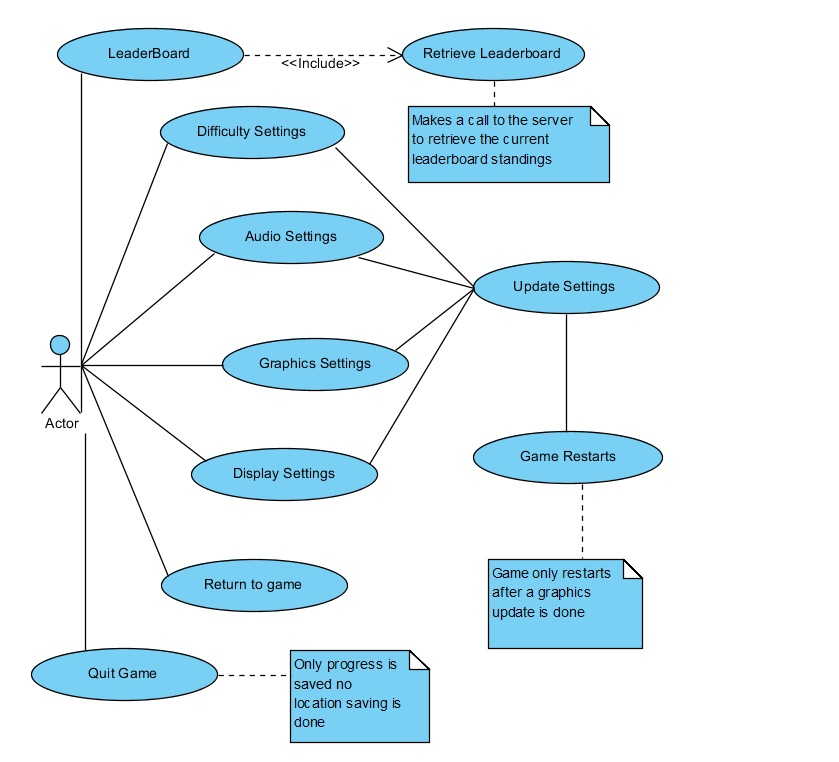
\includegraphics[width=140mm]{UML_Diagram/Use_Case/OptionsScreen_UseCase.jpg}
					\caption{Options Screen}
					\end{figure}
				
				\begin{figure}[H]
					\centering
					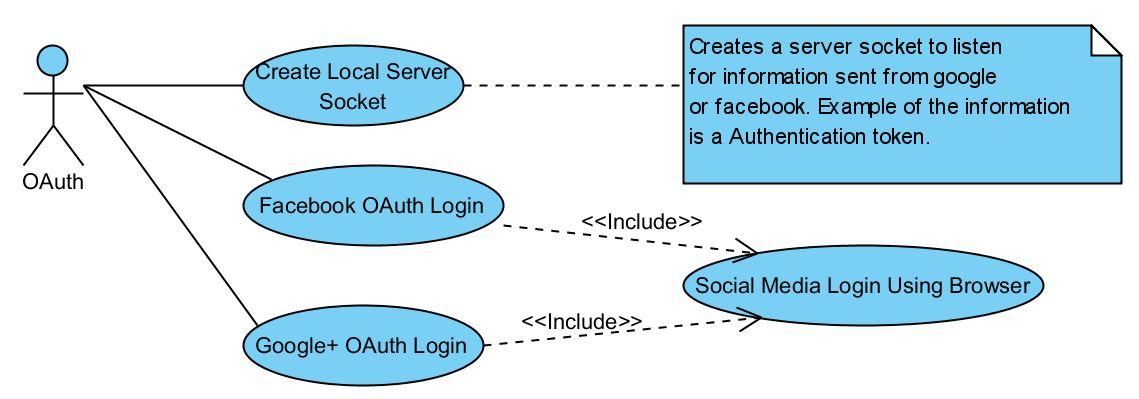
\includegraphics[width=140mm]{UML_Diagram/Use_Case/OAuth.jpg}
					\caption{Login using social media(OAuth)}
					\end{figure}
				
				\vspace{0.2in}
				\subsubsection*{Server Diagrams:}
				\addcontentsline{toc}{subsubsection}{Server Diagrams}
				\vspace{0.2in}
				
					\begin{figure}[H]
					\centering
					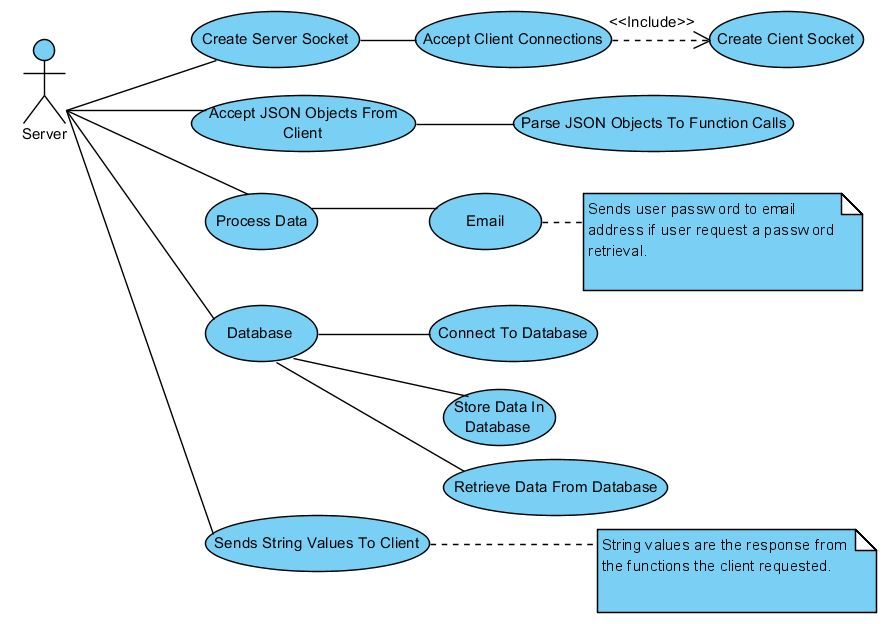
\includegraphics[width=140mm]{UML_Diagram/Use_Case/Server.jpg}
					\caption{Server Functionality}
					\end{figure}
					
					\begin{figure}[H]
					\centering
					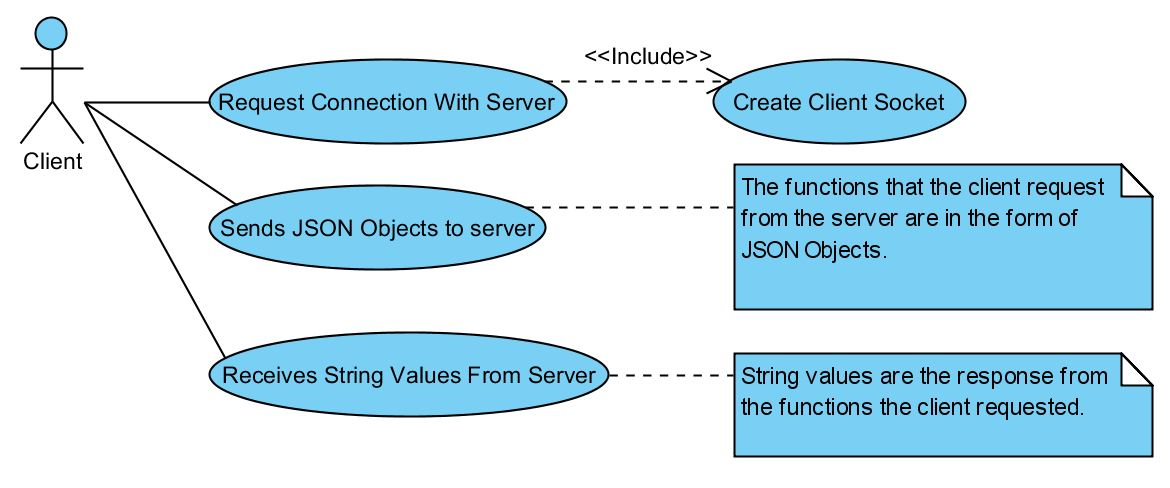
\includegraphics[width=140mm]{UML_Diagram/Use_Case/Client.jpg}
					\caption{User Interaction With Server}
					\end{figure}
				
			\vspace{0.2in}
			\subsection*{Use Case prioritization:}
			\addcontentsline{toc}{subsection}{Use Case prioritization / services contracts}
			\vspace{0.1in}
					
				\subsubsection*{Critical:}
				\addcontentsline{toc}{subsubsection}{Critical}
				\vspace{0.1in}
					
					\begin{itemize}
						\item Update process between frames.
						\item Update of scene elements.
						\item Server Functionality.
						\item User Interaction With Server.
						\item Login using custom login.
						\item Create a new custom account.	
						\item Leaderboard of best all players and scores.					
					\end{itemize}	
					
				\vspace{0.2in}
				\subsubsection*{Important:}
				\addcontentsline{toc}{subsubsection}{Important}
				\vspace{0.2in}
				
					\begin{itemize}
						\item Actions available to player.
						\item Actions available to mobs.
						\item Login using social media(OAuth).
						\item Retrieval of password.
						\item Can change the graphical settings of the game.
						\item Can change audio settings.
					\end{itemize}
				
				\vspace{0.2in}
				\subsubsection*{Nice-To-Have:}
				\addcontentsline{toc}{subsubsection}{Nice-To-Have}
				\vspace{0.2in}
					\begin{itemize}
						\item Update the grpahics while game running.
						\item Change of difficulty settings.
						\item Modibility of the game from external sources.
						\item Addition of more maps.
						\item Multiple types of zombies.
					\end{itemize}
					
			\vspace{0.2in}
			\subsection*{Use Case services contracts:}
			\addcontentsline{toc}{subsection}{Use Case prioritization / services contracts}
			\vspace{0.1in}
				
				\subsubsection*{Game Diagrams:}
				\addcontentsline{toc}{subsubsection}{Game Diagrams}
				\vspace{0.1in}
					
					\hspace{5mm}Update process between frames
					\begin{itemize}
						\item Pre-Conditions: \\
							Game is still running within the main game loop. \\
							Update time is provided from game engine defining the uptime of game. \\
							Player character is not null and initialized to be update. \\
							Mob characters is not null and initialized to be update.
						\item Post-Conditions: \\
							Game scene has updated as defined in update scene elements. \\
							Character action updated as defined in actions of player. \\
							Mobs actions updated as defined in actions of mob.
						\item Request and Results Data Structures \\
							
					\end{itemize}
					
					\vspace{0.1in}
					Actions available to player
					\begin{itemize}
						\item Pre-Condition: \\
							Character handler is not null and initialized. \\
							Character repositioning direction available from the directional keys pressed. \\
							Player animations channel is retrieved from model and can be updated. \\
							Player attack registered for process.
						\item Post-Condition: \\
							Character position has been updated according to direction of movement and movement speed. \\
							Player animation has been set successfully to animations channel with define loop state and play speed. \\
							Player attack action has occurred and processed between player and attacked mob.
						\item Request and Results Data Structures \\
							
					\end{itemize}
					
					\vspace{0.1in}
					Actions available to mobs
					\begin{itemize}
						\item Pre-Condition: \\
							Character handler is not null and initialized. \\
							Character repositioning direction is given from players position. \\
							Mob aggro detection is not null and attach to physics space. \\
							Mob aggro obtained flagged. \\
							Mob aggro loss flagged. \\
							Mob animation channel is retrieved from model and can be updated. \\
							Mob attack registered for process.
						\item Post-Condition: \\
							Character position updated to the direction of player and a distance of the movement speed. \\
							Mob aggro process and state updated for motion and animation loop. \\
							Mob animation has been set successfully to animations channel with define loop state and play speed. \\
							Mob attack action has occurred and processed between mob and player.
						\item Request and Results Data Structures \\
						
					\end{itemize}
					
					\vspace{0.1in}
					Update of scene elements
					\begin{itemize}
						\item Pre-Condition: \\
							Sky control not null and initialized. \\
							Update value provided from game engine of frame time.
						\item Post-Condition: \\
							Sun \& Stars updated by sky control. \\
							Sun direction updated retrieved from sky control and assigned to the light. \\
							Sun on the water updated from the new set light direction. \\
							Time of day updated through sky control.
						\item Request and Results Data Structures \\
						
					\end{itemize}
					
				\vspace{0.2in}
				\subsubsection*{User-interface Diagrams:}
				\addcontentsline{toc}{subsubsection}{User-interface Diagrams}
				\vspace{0.2in}
				
				\vspace{0.1in}
					\hspace{5mm}Creating a custom account
					\begin{itemize}
						\item Pre-Condition: \\
							Client connection to server must be created. \\
							User must not have an existing account registered to the email address he wants to use. \\
							 The username must not be taken by any other player. \\
						\item Post-Condition: \\				
							User must be logged into the game. \\
							User's details must be stored to the database. \\
							User's username and score must be displayed on the leaderboard. 
						\item Request and Results Data Structures \\
						
					\end{itemize}
					
				\vspace{0.1in}Login using a custom account
					\begin{itemize}
						\item Pre-Condition: \\
							Client connection to server must be created. \\				
							User must have a registered custom account. \\
						\item Post-Condition: \\
							User must be logged in and game must be running. \\
							Username must be displayed on the leaderboard. \\			
						\item Request and Results Data Structures \\
						
					\end{itemize}

				\vspace{0.1in}Retrieval of custom account password
					\begin{itemize}
						\item Pre-Condition: \\
							Client connection to server must be created. \\
							User must have a registerd username and email linked to their custom account. \\ 
						\item Post-Condition: \\
							Email is sent to registered email address. \\
							User is taken back to the login screen. \\
						\item Request and Results Data Structures \\
						
					\end{itemize}
									
				\vspace{0.1in}Leaderboard updates
					\begin{itemize}
						\item Pre-Condition: \\
							User must be logged in. \\ 
							User must kill a zombie. \\
						\item Post-Condition: \\
							Score updated on leaderboard screen. \\						
						\item Request and Results Data Structures \\
						
					\end{itemize}					
														
				\vspace{0.1in}Loading Screen
					\begin{itemize}
						\item Pre-Condition: \\
							User must have a successful login. \\
						\item Post-Condition: \\
						 	Game is loaded and user can play. \\
						\item Request and Results Data Structures \\
						
					\end{itemize}	
								
				\vspace{0.1in}Options Menu
					\begin{itemize}
						\item Pre-Condition: \\
							User must be logged into the game. \\
							User must hit the escape key. \\
						\item Post-Condition: \\
							Options menu screen must appear. \\
							Mouse must be visible. \\
							Selections must be selectable. \\
						\item Request and Results Data Structures \\
						
					\end{itemize}	
									
				\vspace{0.1in}Graphics Settings tab
					\begin{itemize}
						\item Pre-Condition: \\
							Options Menu must be open. \\
							Graphics settings must be selected. \\
						\item Post-Condition: \\
							Graphics settings are displayed. \\
							Previous choices must be already ticked. \\
						\item Request and Results Data Structures \\
						
					\end{itemize}									
									
				\vspace{0.1in}Quiting the game
					\begin{itemize}
						\item Pre-Condition: \\
							User must be in the options menu or login screen. \\
							User must select quit game. \\ 
						\item Post-Condition: \\
							Game must close and user returned to previous position on desktop. \\
						\item Request and Results Data Structures \\
						
					\end{itemize}
														
				
				\vspace{0.1in}Login using social media(OAuth)
					\begin{itemize}
						\item Pre-Condition: \\
							User must have a google or facebook account. \\
							User must login with his facebook or google profile. \\
							User must grant permission for the game to access social information.
						\item Post-Condition: \\
							User must be logged in the game. \\
							Server must have an access token of the social media used to log in.			
						\item Request and Results Data Structures \\
						
					\end{itemize}
				
				\newpage
				\subsubsection*{Server Diagrams:}
				\addcontentsline{toc}{subsubsection}{Server Diagrams}
				\vspace{0.2in}
				
				\vspace{0.1in}
					\hspace{5mm}Server Functionality
					\begin{itemize}
						\item Pre-Condition: \\
							Server socket needs to be created. \\
							Connection from server to database needs to be established. \\
							Server needs to listen for incoming connection.
						\item Post-Condition: \\
							Server needs to accept all incoming connection from the game. \\
							Server must handle all functions requested from user(game).\\
							Server needs to store and retrieve data from the database.			
						\item Request and Results Data Structures \\
							All function request from the user(game) are JSON strings. 
						
					\end{itemize}
					
					\vspace{0.1in}
					User Interaction With Server
					\begin{itemize}
						\item Pre-Condition: \\
							Client socket needs to be created. \\
							Client socket must connect with server. \\
							Client needs to send data to the server. 
						\item Post-Condition: \\
							Client must be connected to server. \\
							Client needs to receive data from server.			
						\item Request and Results Data Structures \\
							All data sent and received between server and client are JSON strings.						
					\end{itemize}
					
			\vspace{0.2in}
			\subsection*{Process specifications:}
			\addcontentsline{toc}{subsection}{Process specifications}
			\vspace{0.1in}
			
			\begin{figure}[H]
			\centering
			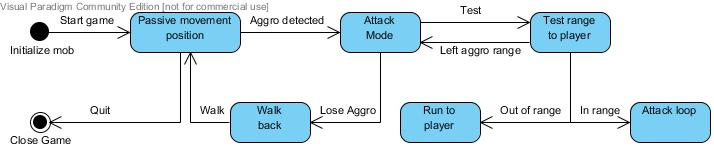
\includegraphics[width=180mm]{UML_Diagram/State/Mob_Aggro.jpg}
			\caption{Enemy aggression cycle}
			\label{overflow}
			\end{figure}
			
			Enemy aggression cycle depicts the phases an enemy player goes through to decide in which state it is in and how to react regarding that state.
			
				\begin{figure}[H]
			\centering
			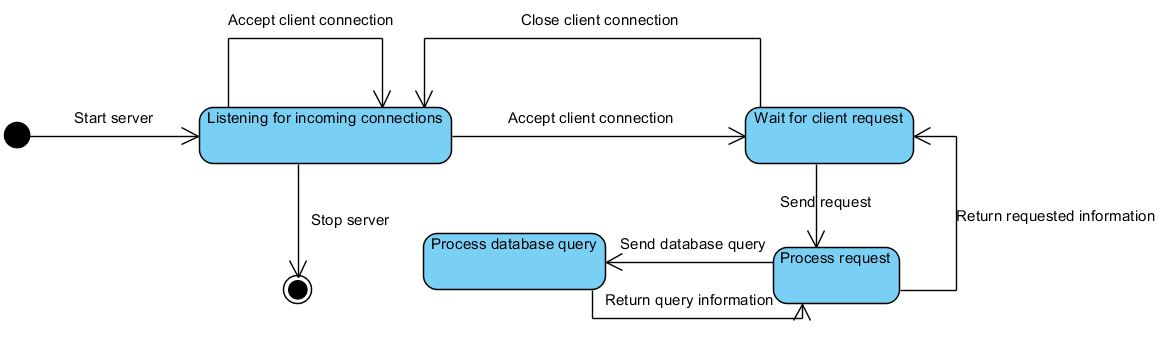
\includegraphics[width=180mm]{UML_Diagram/State/Server_State_Diagram.jpg}
			\caption{Server cycle}
			\label{overflow}
			\end{figure}
			
		\begin{figure}[H]
			\centering
			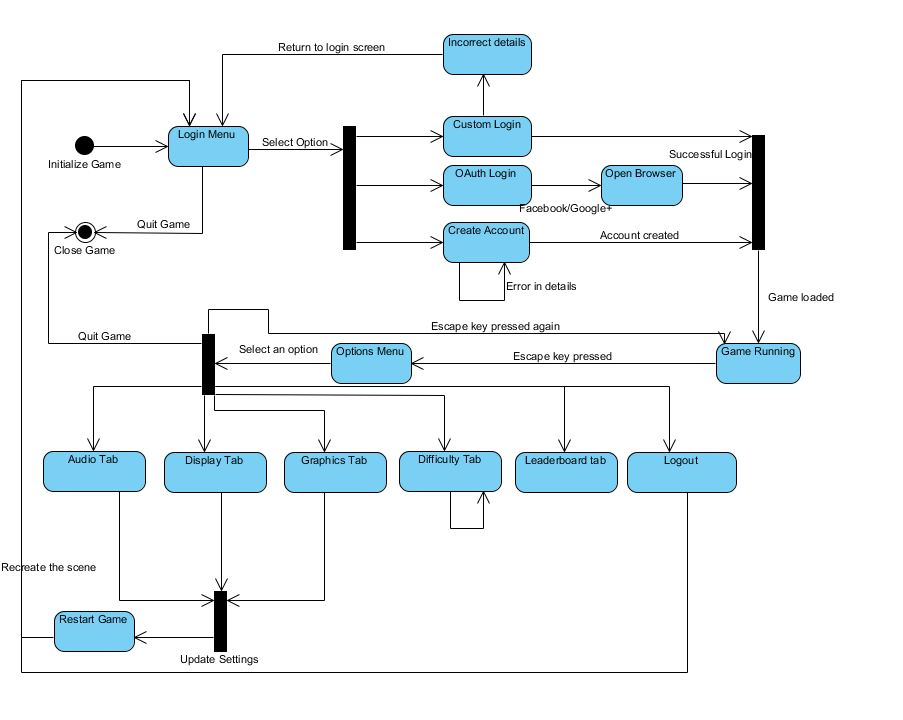
\includegraphics[width=180mm]{UML_Diagram/State/GUI_State.jpg}
			\caption{User-Interface cycle}
			\label{overflow}
			\end{figure}
			
			\vspace{0.2in}
			\subsection*{Domain Objects:}
			\addcontentsline{toc}{subsection}{Domain Objects}
			\vspace{0.1in}
			
				\vspace{0.2in}
				\subsubsection*{Class Diagrams:}
				\addcontentsline{toc}{subsubsection}{Class Diagrams}
				\vspace{0.1in}
				
					\begin{figure}[H]
					\centering
					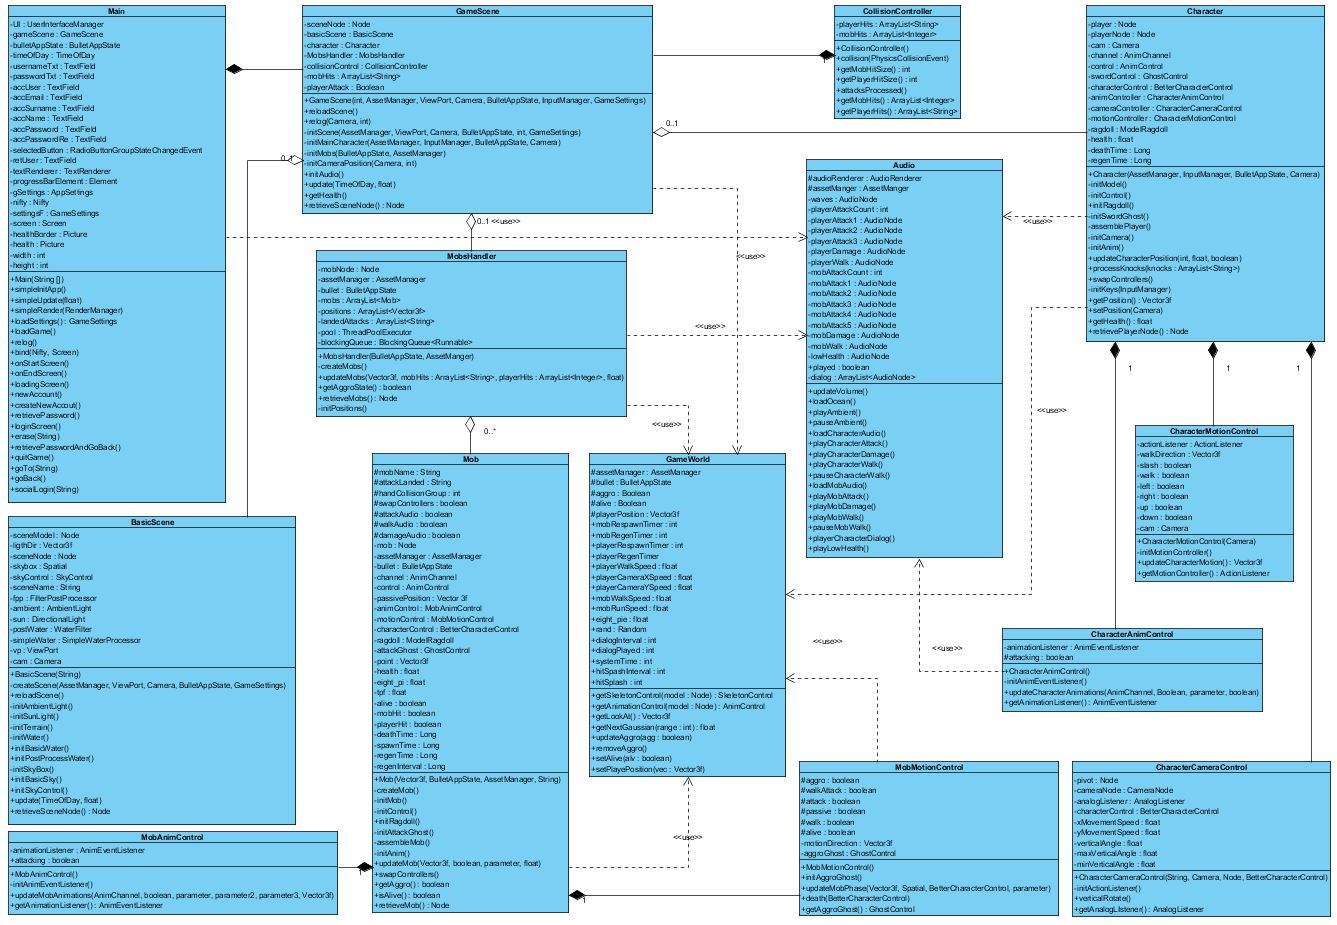
\includegraphics[width=180mm]{UML_Diagram/Class/Game_Classes.jpg}
					\caption{Game level class diagram}
					\label{overflow}
					\end{figure}
					
					\begin{figure}[H]
					\centering
					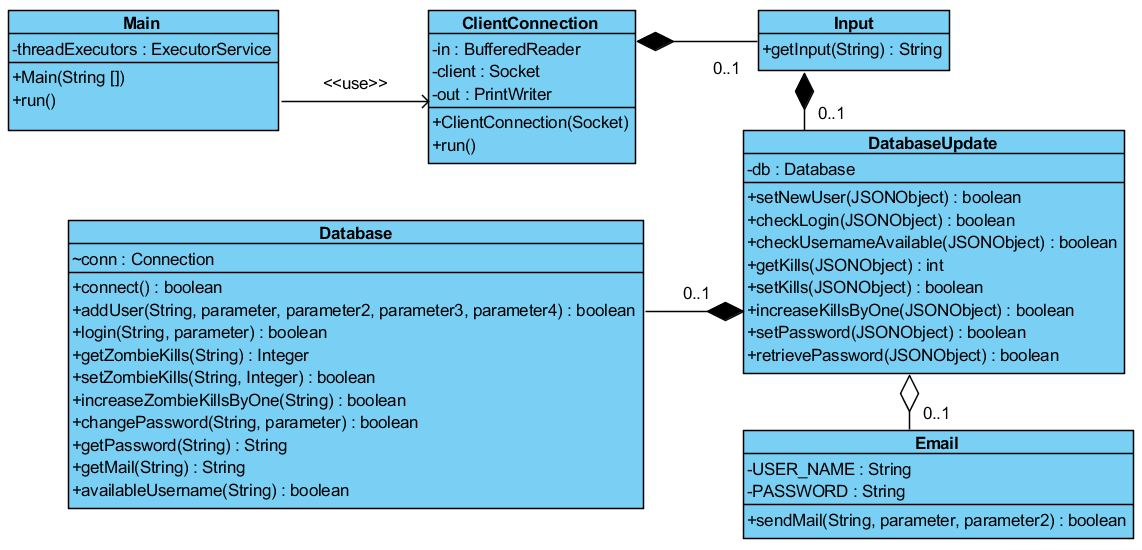
\includegraphics[width=180mm]{UML_Diagram/Class/Server_Classes.jpg}
					\caption{Server level class diagram}
					\label{overflow}
					\end{figure}
					
					\begin{figure}[H]
					\centering
					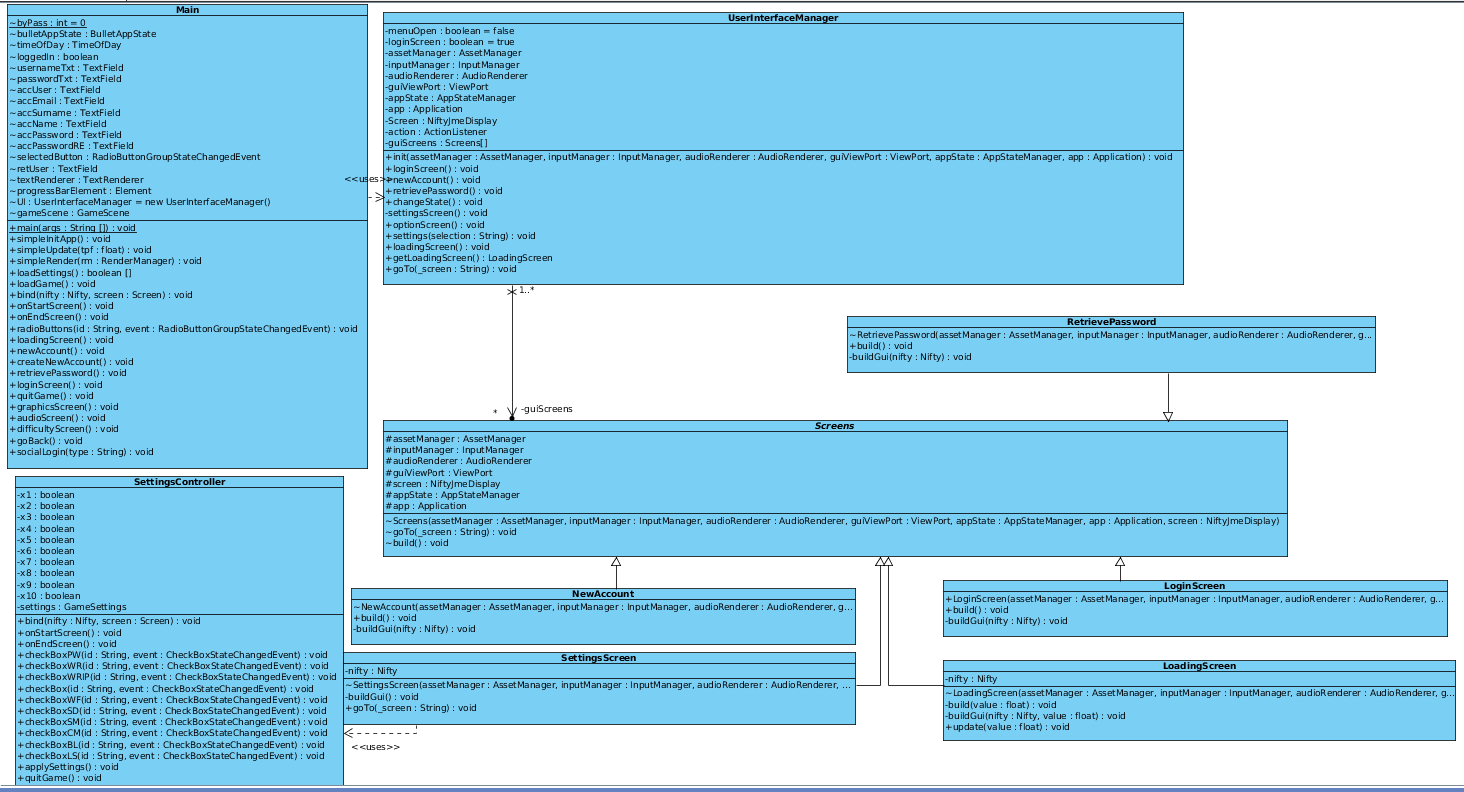
\includegraphics[width=180mm]{UML_Diagram/Class/GUI_Classes.jpg}
					\caption{User-Interface class diagram}
					\label{overflow}
					\end{figure}
					
				\vspace{0.2in}	
				\subsubsection*{ERD Diagrams:}
				\addcontentsline{toc}{subsubsection}{ERD Diagrams}
				\vspace{0.1in}
				
					\begin{figure}[H]
					\centering
					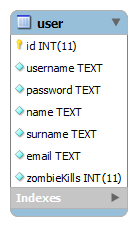
\includegraphics[width=40mm]{UML_Diagram/ERD/Database.png}
					\caption{Game level class diagram}
					\label{overflow}
					\end{figure}
					
					
		\vspace{0.2in}
		
		\section*{\colorbox{blue}{\makebox[\textwidth-2\fboxsep][l]{\bfseries\color{white} Application Design }}} \addcontentsline{toc}{section}{Application Design}
		\vspace{0.1in}
		
		\begin{figure}[H]
		\centering
		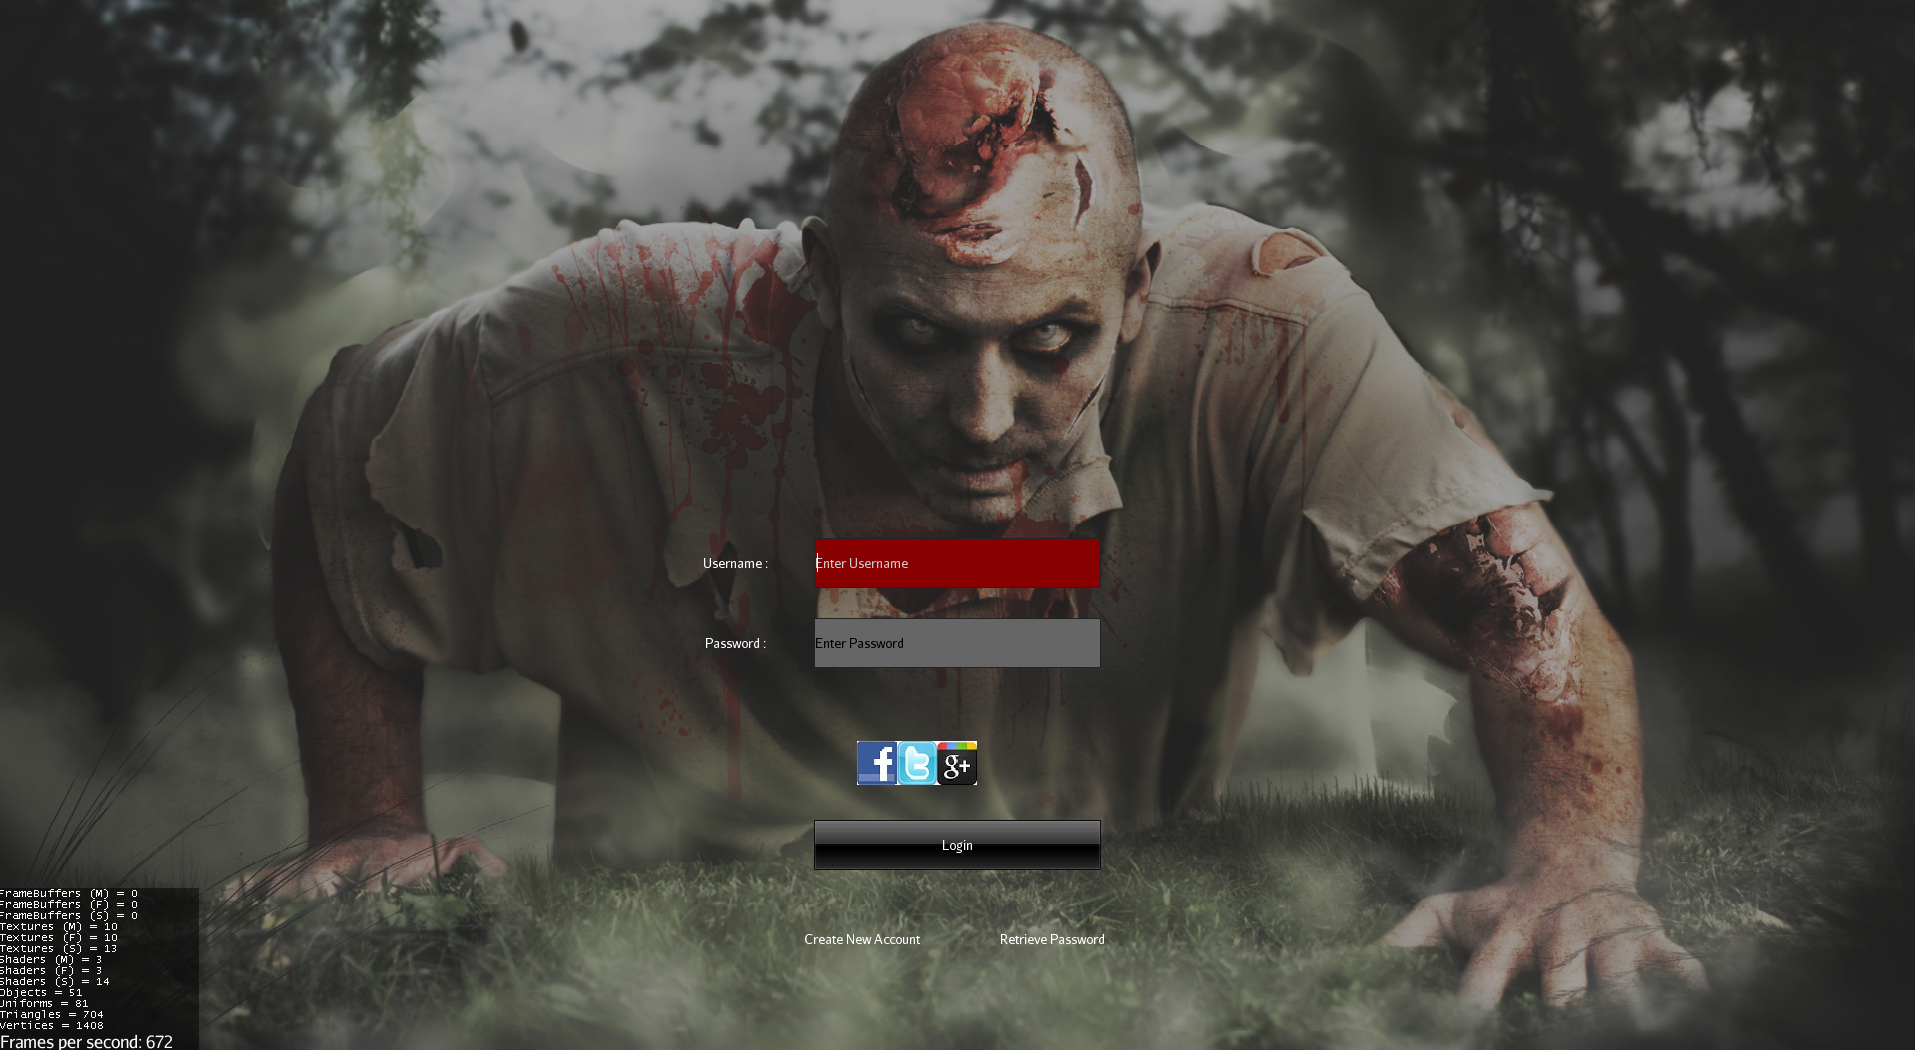
\includegraphics[width=130mm]		{GUI_ScreenShots/LoginScreen.jpg}
		\caption{Login Screen}
		\end{figure}
		

		
		\begin{figure}[H]
		\centering
		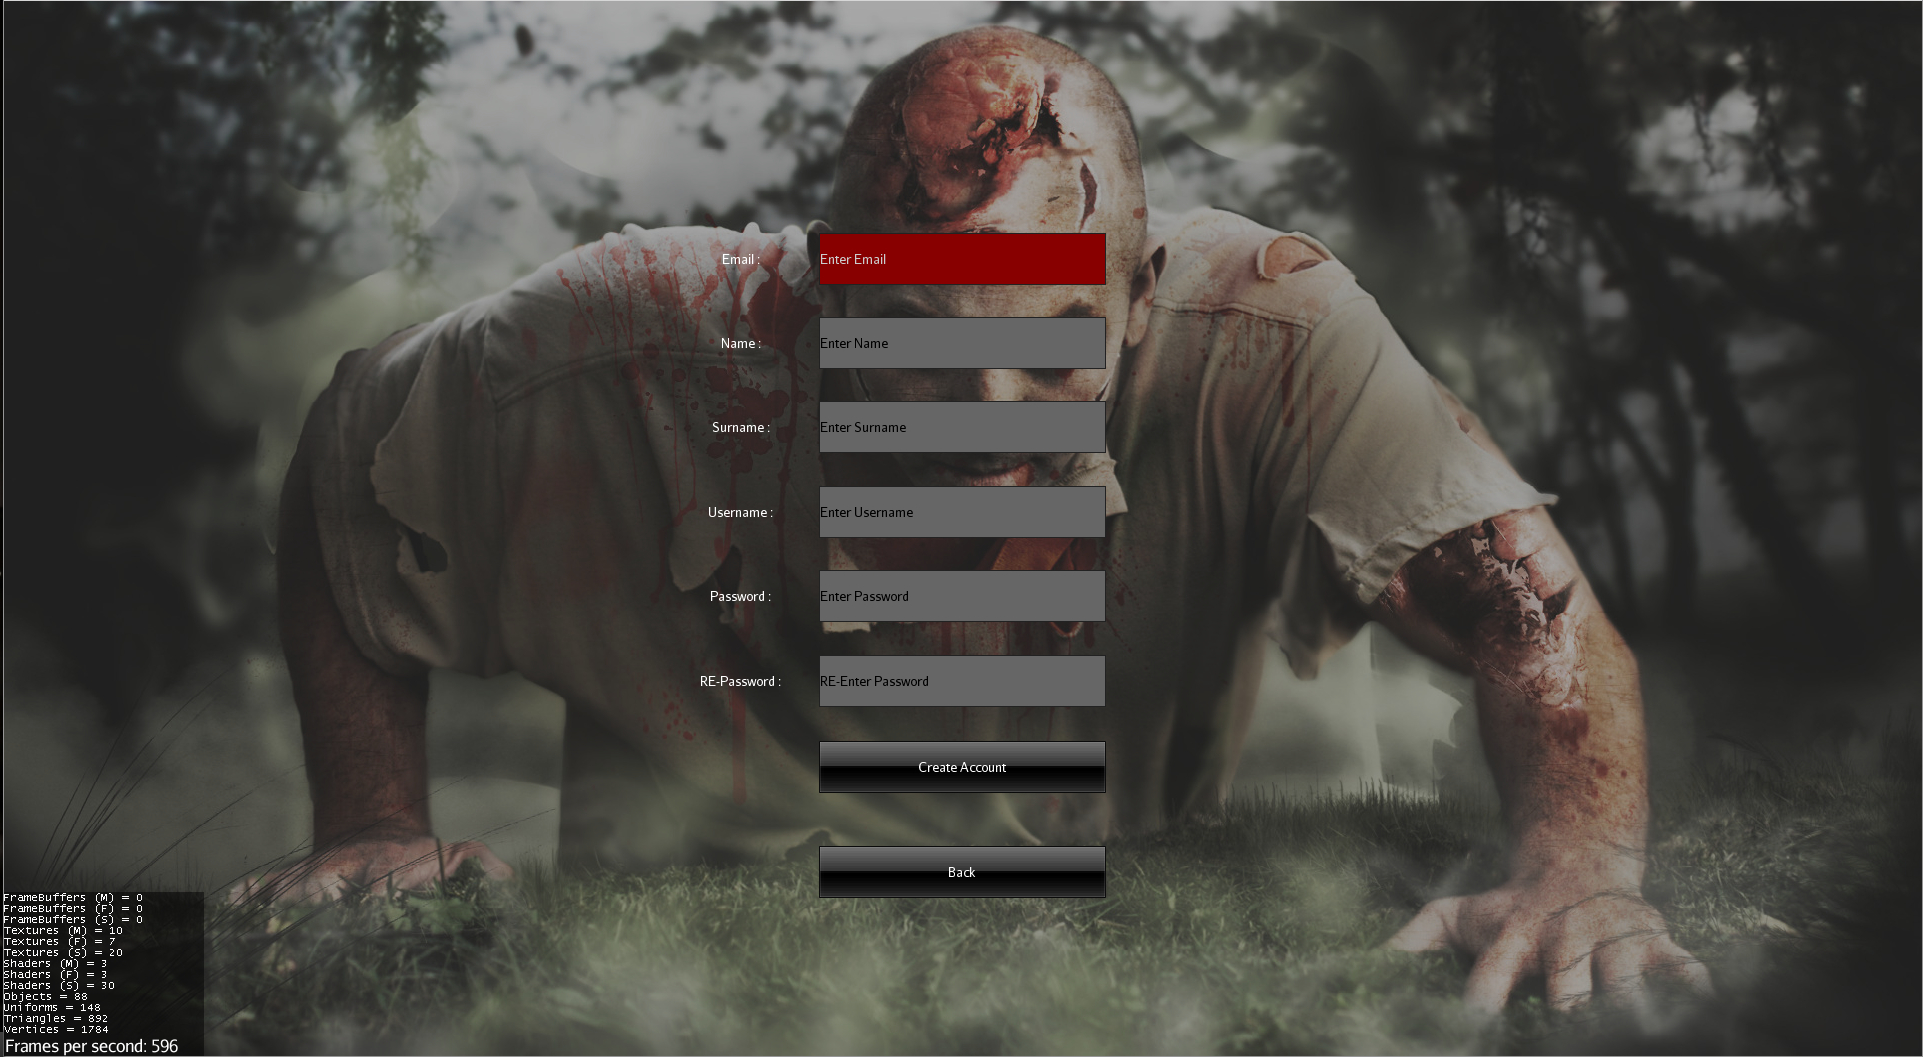
\includegraphics[width=130mm]{GUI_ScreenShots/CreateAccount.jpg}
		\caption{Create Account Screen}
		\end{figure}
		

			
		\begin{figure}[H]
		\centering
		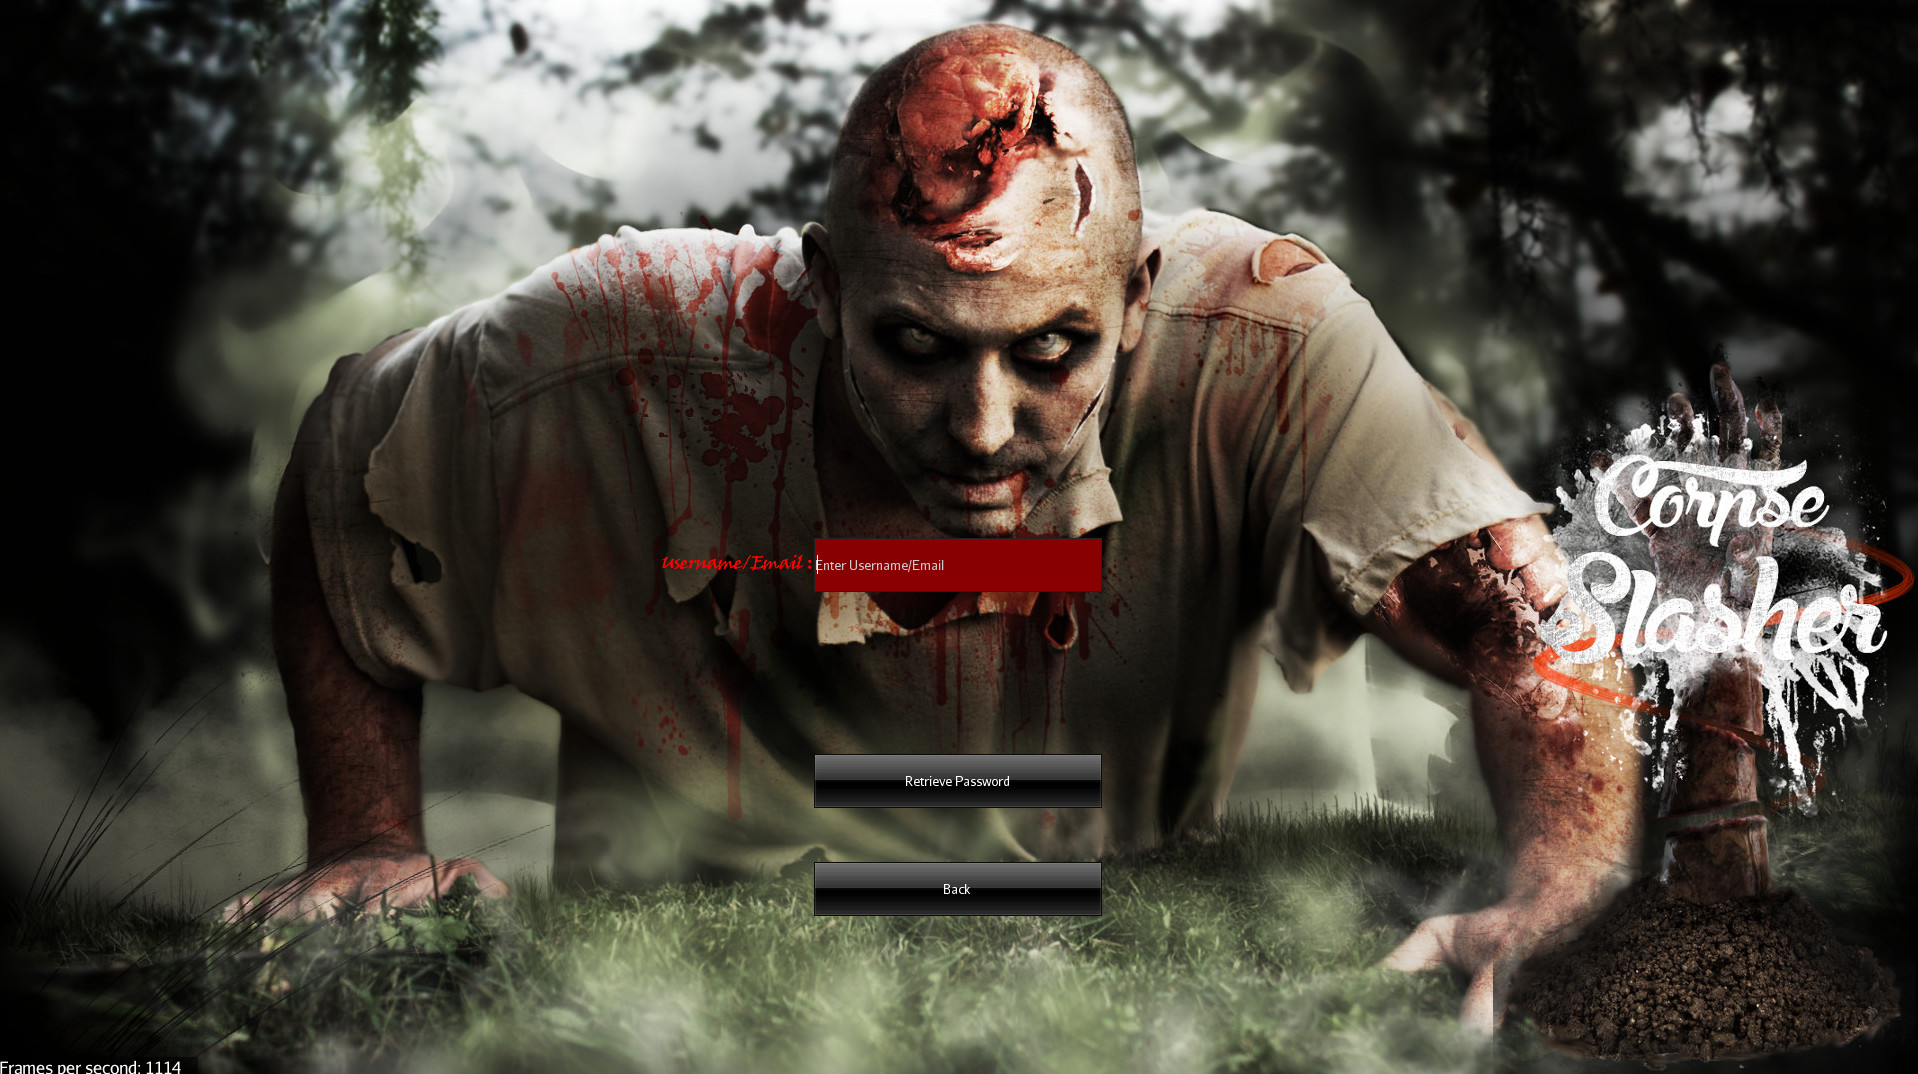
\includegraphics[width=130mm]{GUI_ScreenShots/RetrievePassword.jpg}
		\caption{Retrieve Password Screen}
		\end{figure}
		
			
		\begin{figure}[H]
		\centering
		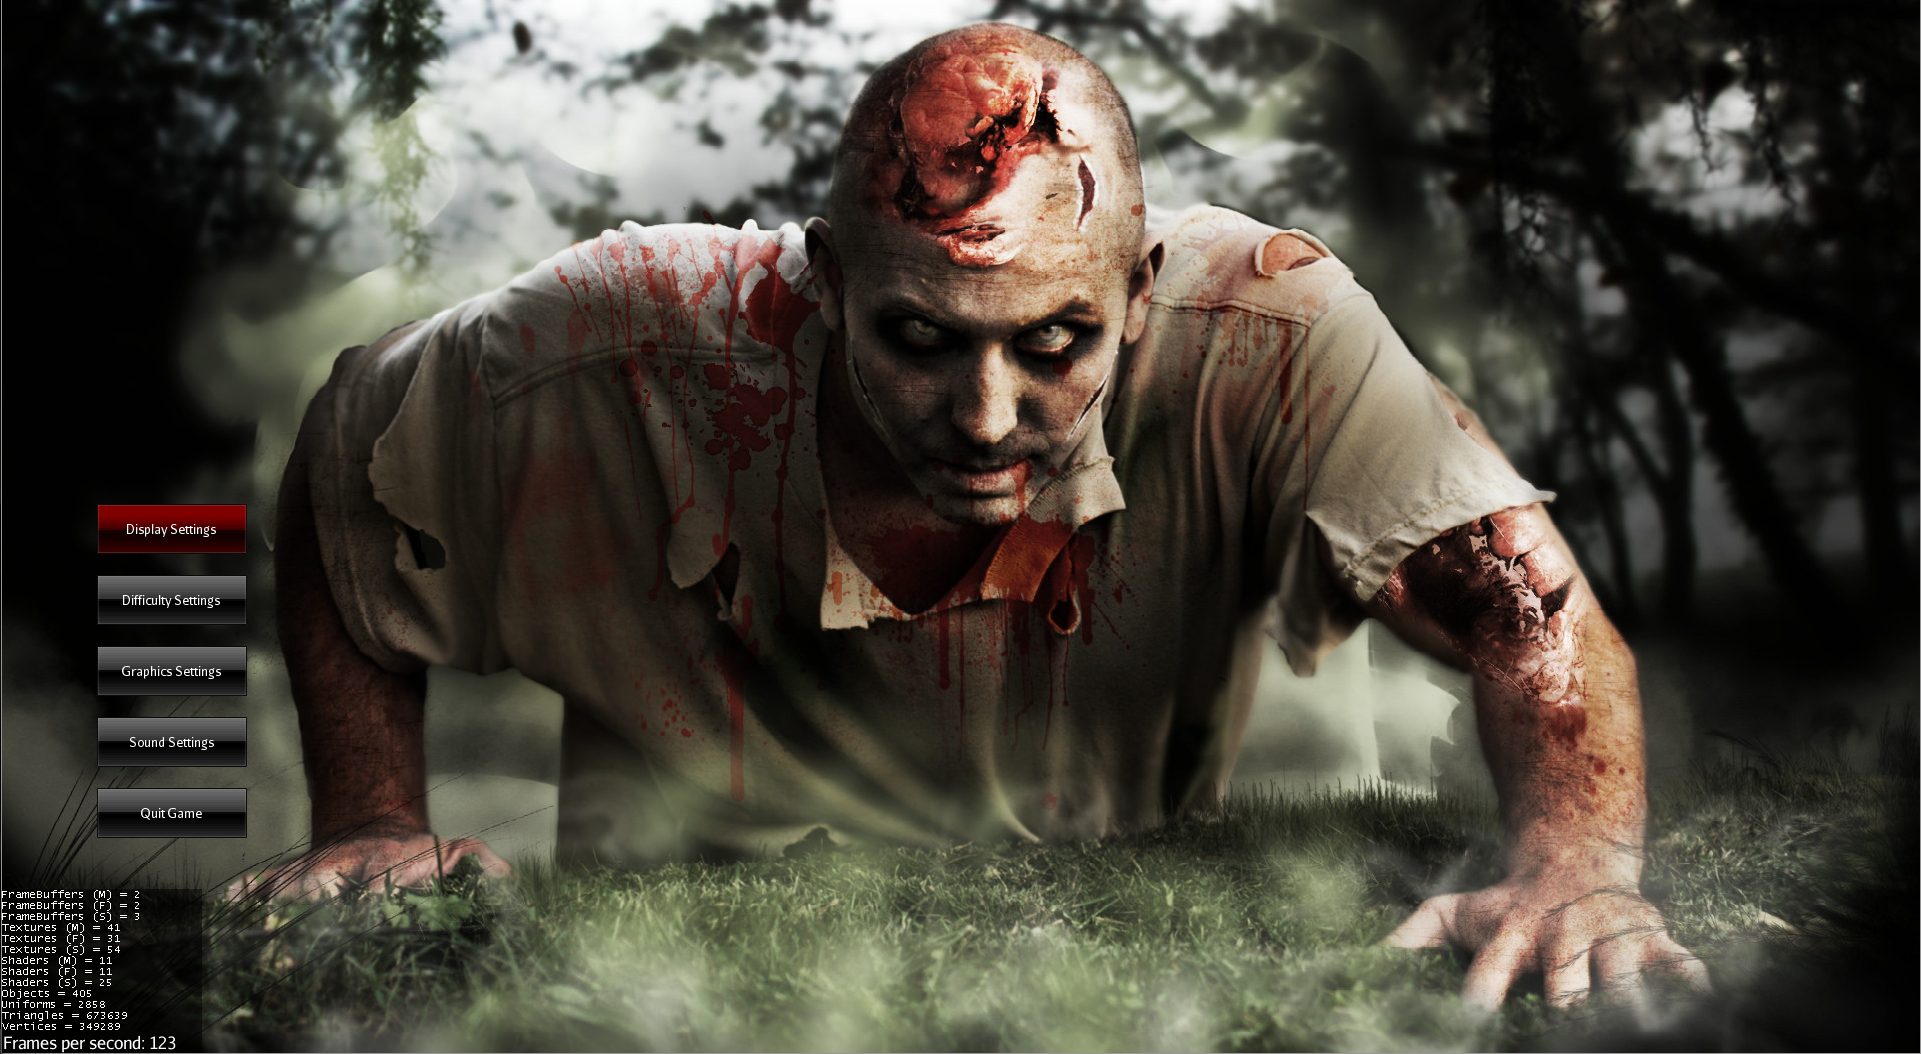
\includegraphics[width=130mm]{GUI_ScreenShots/OptionsScreen.jpg}
		\caption{Options Screen}
		\end{figure}
		
			
		\begin{figure}[H]
		\centering
		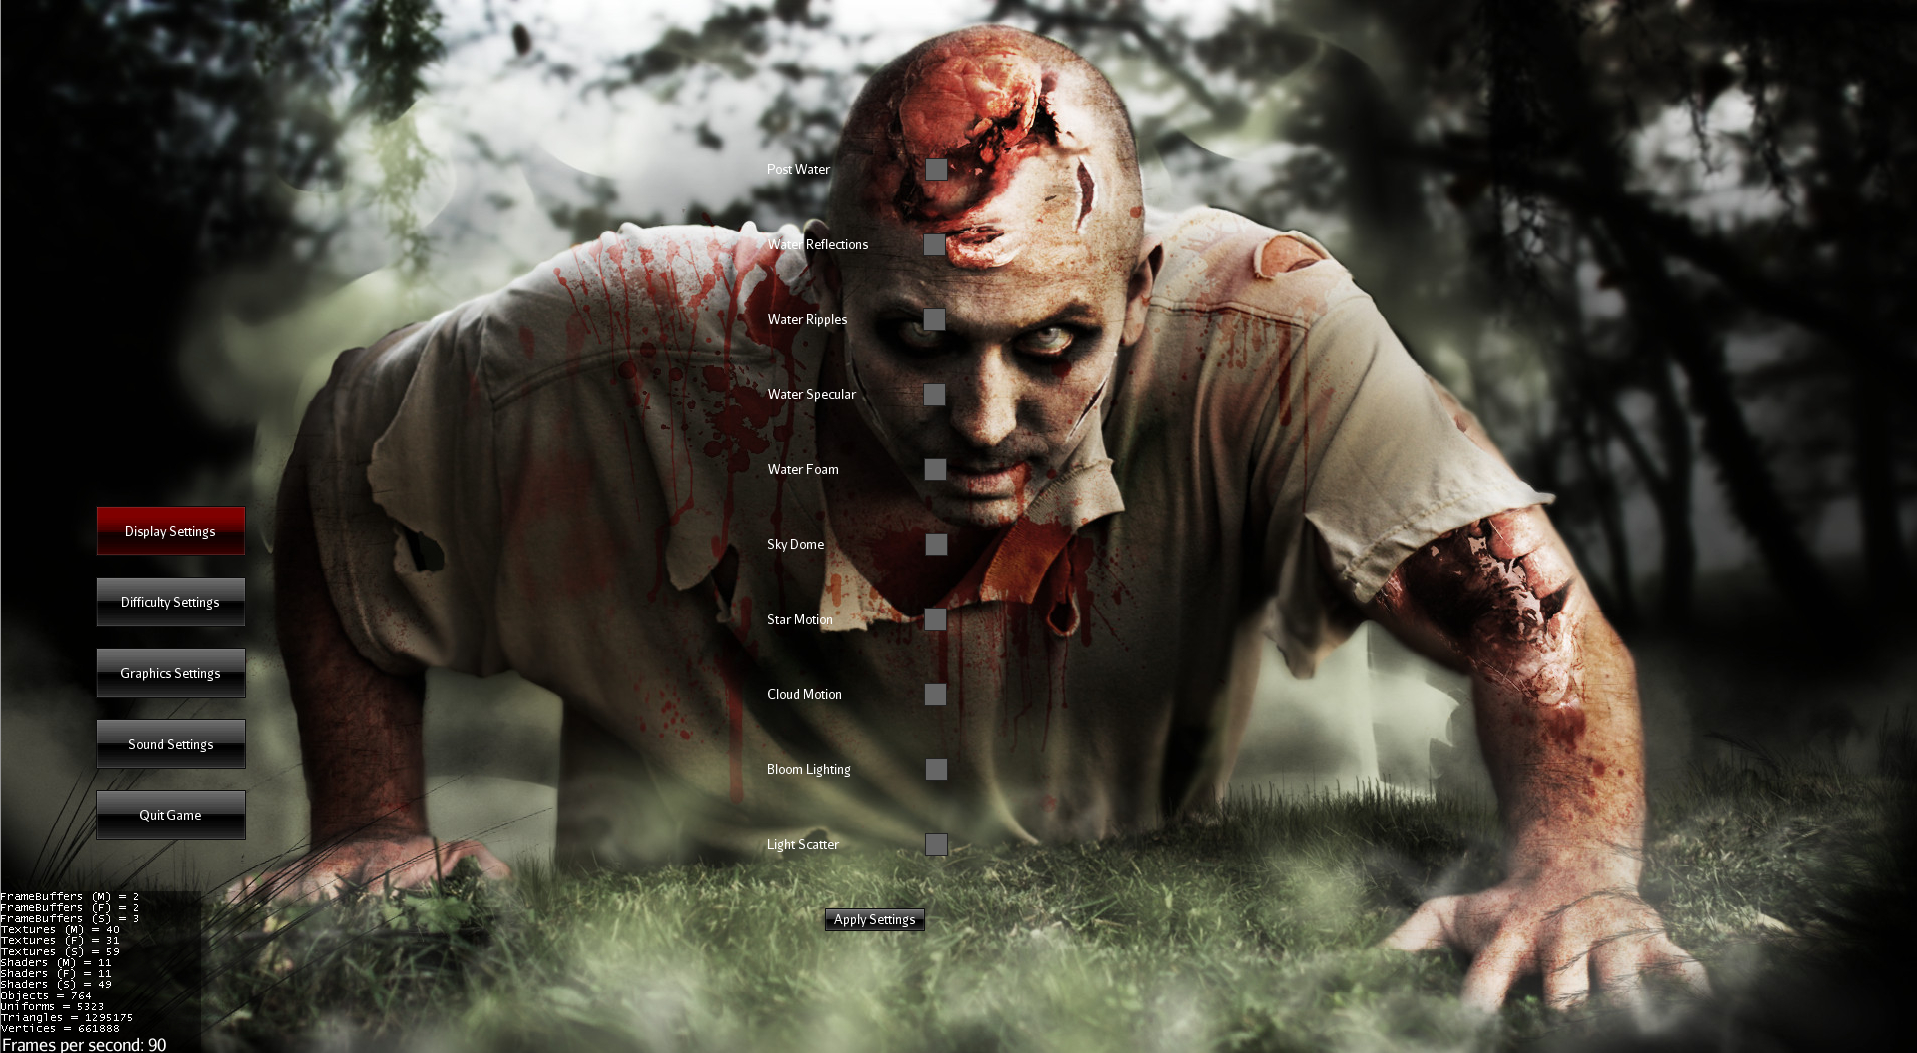
\includegraphics[width=130mm]{GUI_ScreenShots/GraphicsSettings.jpg}
		\caption{Graphics Settings tab}
		\end{figure}
		
		
		\vspace{0.2in}
		
		\section*{\colorbox{blue}{\makebox[\textwidth-2\fboxsep][l]{\bfseries\color{white} Code Documentation }}} \addcontentsline{toc}{section}{Code Documentation}
		\vspace{0.1in}
		
			\subsection*{Game Main:}
			\addcontentsline{toc}{subsection}{Game Main}
			\vspace{0.1in}
				
				\begin{itemize}
					\item 	All Implemented Interfaces: \\
							com.jme3.system.SystemListener, de.lessvoid.nifty.screen.ScreenController
					\item	Field Summary
							\begin{itemize}
								\item	(package private) de.lessvoid.nifty.controls.TextField	accEmail 
								\item	(package private) de.lessvoid.nifty.controls.TextField	accName 
								\item	(package private) de.lessvoid.nifty.controls.TextField	accPassword 
								\item	(package private) de.lessvoid.nifty.controls.TextField	accPasswordRE 
								\item	(package private) de.lessvoid.nifty.controls.TextField	accSurname 
								\item	(package private) de.lessvoid.nifty.controls.TextField	accUser 
								\item	(package private) com.jme3.bullet.BulletAppState	bulletAppState 
								\item	(package private) static int	byPass 
								\item	(package private) GameScene	gameScene 
								\item	(package private) boolean	loggedIn 
								\item	(package private) de.lessvoid.nifty.controls.TextField	passwordTxt 
								\item	(package private) de.lessvoid.nifty.elements.Element	progressBarElement 
								\item	(package private) de.lessvoid.nifty.controls.TextField	retUser 
								\item	(package private) de.lessvoid.nifty.controls.RadioButtonGroupStateChangedEvent	selectedButton 
								\item	(package private) de.lessvoid.nifty.elements.render.TextRenderer	textRenderer 
								\item	(package private) jme3utilities.TimeOfDay	timeOfDay 
								\item	(package private) UserInterfaceManager	UI 
								\item	(package private) de.lessvoid.nifty.controls.TextField
							\end{itemize} 
					\item	Fields inherited from class com.jme3.app.SimpleApplication \\
							flyCam, fpsText, guiFont, guiNode, INPUT\_MAPPING\_CAMERA\_POS, \\ INPUT\_MAPPING\_EXIT, INPUT\_MAPPING\_HIDE\_STATS, INPUT\_MAPPING\_MEMORY, \\ rootNode, showSettings
					\item	Fields inherited from class com.jme3.app.Application \\
							assetManager, audioRenderer, cam, context, guiViewPort, inputEnabled, inputManager, joyInput, keyInput, listener, mouseInput, paused, pauseOnFocus, renderer, renderManager, settings, speed, stateManager, timer, touchInput, viewPort
					\item	Constructor Summary \\
							Main()
					\item	Methods inherited from class com.jme3.app.SimpleApplication \\
							getFlyByCamera, getGuiNode, getRootNode, initialize, isShowSettings, loadGuiFont, setDisplayFps, setDisplayStatView, setShowSettings, start, update
					\item	Methods inherited from class com.jme3.app.Application \\
							createCanvas, destroy, destroyInput, enqueue, gainFocus, getAssetManager, getAudioRenderer, getCamera, getContext, getGuiViewPort, getInputManager, getListener, getRenderer, getRenderManager, getStateManager, getTimer, getViewPort, handleError, isPauseOnLostFocus, loseFocus, requestClose, reshape, restart, runQueuedTasks, setAssetManager, setPauseOnLostFocus, setSettings, setTimer, start, startCanvas, startCanvas, stop, stop
					\item	Method Detail
							\begin{itemize}
								\item	main \\
										public static void main(java.lang.String[] args)
								\item	simpleInitApp \\
										public void simpleInitApp() \\ \\
										This function only gets called once. Use this function to create the login screen where after the scene will be compiled during loading screen. \\ \\
										Specified by: \\
										simpleInitApp in class com.jme3.app.SimpleApplication
								\item	simpleUpdate \\
										public void simpleUpdate(float tpf) \\ \\
										Overrides: \\
										simpleUpdate in class com.jme3.app.SimpleApplication
								\item	simpleRender \\
										public void simpleRender(com.jme3.renderer.RenderManager rm) \\ \\
										Overrides: \\
										simpleRender in class com.jme3.app.SimpleApplication
								\item	loadSettings
										public boolean[] loadSettings() \\ \\
										Returns: \\
										an array of booleans checking which settings to activate. Loading the settings based on the .txt file
								\item	loadGame \\
										public void loadGame() \\ \\
										This function assembles all the game elements in order to render the game.
								\item	bind \\
										public void bind(de.lessvoid.nifty.Nifty nifty,de.lessvoid.nifty.screen.Screen screen) \\ \\
										Specified by:
										bind in interface de.lessvoid.nifty.screen.ScreenController \\ \\
										Parameters:
										nifty - the object containing all the components of the GUI \\
										screen - the actual screen panel of the nifty GUI at the binding of the create \\ account screen all the appropriate text field's data are collected and checked
								\item	onStartScreen \\
										public void onStartScreen() \\ \\
										Specified by: \\
										onStartScreen in interface de.lessvoid.nifty.screen.ScreenController
								\item	onEndScreen \\
										public void onEndScreen() \\ \\
										Specified by: \\
										onEndScreen in interface de.lessvoid.nifty.screen.ScreenController
								\item	radioButtons \\
										public void radioButtons(java.lang.String id, de.lessvoid.nifty.controls.RadioButtonGroupStateChangedEvent event) \\ \\
										Parameters: \\
										id - the ID of radio button selected \\
										event - the state of the selected radio button on a state change the button event is updated
								\item	loadingScreen
										public void loadingScreen() \\ \\
										After a successful login the loading screen is loaded and the game starts to load
								\item	newAccount \\
										public void newAccount() \\ \\
										Changes the screen to the new account screen
								\item	createNewAccount \\
										public void createNewAccount() \\ \\
										Checks all the appropriate fields whther they are valid and then adds the data to the database and logins in
								\item	retrievePassword \\
										public void retrievePassword() \\ \\
										Goes to the retrieve password screen
								\item	loginScreen \\
										public void loginScreen() \\
										Goes to the login screen
								\item	quitGame \\
										public void quitGame() \\ \\
										Quits the game
								\item	graphicsScreen \\
										public void graphicsScreen() \\ \\
										Goes to the graphics settings from the option screen
								\item	audioScreen \\
										public void audioScreen() \\ \\
										Goes to the audio settings from the option screen
								\item	difficultyScreen
										public void difficultyScreen() \\ \\
										Goes to the difficulty settings from the option screen
								\item	goBack \\
										public void goBack() \\ \\
										Goes back to the login screen
								\item	socialLogin \\
										public void socialLogin(java.lang.String type) \\ \\
										Logins in via the selected social media
							\end{itemize}
				\end{itemize}
				
			\vspace{0.2in}
			\subsection*{Game documentation:}
			\addcontentsline{toc}{subsection}{Game documentation}
			\vspace{0.1in}
			
				\subsubsection*{GameScene:}
				\addcontentsline{toc}{subsubsection}{GameScene}
				\vspace{0.1in}
					\begin{itemize}
						\item	Field Summary
								\begin{itemize}
									\item	private BasicScene	basicScene 
									\item	private Character	character 
									\item	private MobsHandler	mobHandler 
									\item	private com.jme3.scene.Node	sceneNode 
								\end{itemize}
						\item	Constructor Detail \\
								public GameScene(int selectedMap, \\ com.jme3.asset.AssetManager assestManager, com.jme3.renderer.ViewPort viewPort, \\ com.jme3.renderer.Camera cam, com.jme3.bullet.BulletAppState bullet, \\ com.jme3.input.InputManager inMan, \\ LoadingScreen ui, \\ GameSettings settings) \\ \\
								GameScene will combine all the entities of the entire game into a node for a reverance point for the game engine. \\ \\
								Parameters: \\
								selectedMap - - the desired map to load. \\
								assetManager - - Assetmanager passed through from main game. \\
								viewPort - - ViewPort required for water, contains position of camara.
						\item	Method Detail
								\begin{itemize}
									\item	initScene \\
											private void initScene(com.jme3.asset.AssetManager assestManager, \\
		             com.jme3.renderer.ViewPort viewPort, \\
		             com.jme3.renderer.Camera cam, \\
		             com.jme3.bullet.BulletAppState bullet, \\
		             int map, \\
		             LoadingScreen ui, \\
		             GameSettings settings) \\ \\
											initScene will retrieve and combine all the variase assets that will make up the entire scene. \\ \\
											Parameters: \\
											assestManager - - AssestManager for loading all required models and textures. \\
											viewPort - - ViewPort required for post processing filter: Water. \\
											cam - - Camera required for the sky controller to update the postion of assets. \\
											bullet - - BulletAppState to add collision detection to the terrain and its added assest. \\
											map - - Corresponding scene number to assign the required terrain.
									\item	initMainCharacter \\
											private void initMainCharacter(com.jme3.asset.AssetManager assMan, \\
		                     com.jme3.input.InputManager inMan, \\
		                     com.jme3.bullet.BulletAppState bullet, \\
		                     com.jme3.renderer.Camera cam) \\ \\
											initMainCharacter will load the main player model, add it to a character handler to be able to add gravity and move it around, also add the key and mouse functionality to control and update it the model and camera positions. \\ \\
											Parameters: \\
											assMan - - AssetManager to be able to load models and textures. \\
											inMan - - InputManager for adding key and mouse binding to be triggered. \\
											bullet - - BulletAppState to add the model to the physics handler.
									\item	initMobs \\
											private void initMobs(com.jme3.bullet.BulletAppState bullet, \\
		            com.jme3.asset.AssetManager assMan) \\ \\
											initMobs will be responsible for creating all the mobs at specified positions also update its position, animation and aggression control. \\ \\
											Parameters: \\
											bullet - - BulletAppState for add collision boxes and controllers. \\
											assMan - - AssetManager for loading the model.
									\item	initCameraPosition \\
											private void initCameraPosition(com.jme3.renderer.Camera cam, \\
		                      int map) \\ \\
											initCameraPosition will be used the multiple maps are create to define the correct camera position. \\ \\
											Parameters: \\
											cam - - Camera from main game. \\
											map - - The scene to be loaded.
									\item	update \\
											public void update(com.jme3.renderer.Camera cam, \\
		          jme3utilities.TimeOfDay tod, \\
		          float tpf) \\ \\
											update will update the all the corrisponding assets of the game. From light direction, time of day, water light reflection, character position. \\ \\
											Parameters: \\
											cam - - Camera to be use for updating camera position. \\
											tod - - TimeOfDay to update the skycontrol time of day. \\
											tpf - - Update value of time between frames.
									\item	retrieveSceneNode \\
											public com.jme3.scene.Node retrieveSceneNode() \\ \\
											retrieveSceneNode to obtain the node that contains all the assests of the scene which will be added to the rootNode for it to be renderable. \\
											Returns: \\
											sceneNode consisting of the entire scene.
								\end{itemize}
					\end{itemize}
				
				\vspace{0.2in}
				\subsubsection*{BasicScene:}
				\addcontentsline{toc}{subsubsection}{BasicScene}
				\vspace{0.1in}
					\begin{itemize}
						\item	Field Summary
								\begin{itemize}
									\item	private com.jme3.light.AmbientLight	ambient
									\item	private com.jme3.post.FilterPostProcessor	fpp
									\item	private com.jme3.math.Vector3f	lightDir
									\item	private com.jme3.scene.Spatial	sceneModel
									\item	private java.lang.String	sceneName
									\item	private com.jme3.scene.Node	sceneNode
									\item	private GameSettings	settings
									\item	private jme3utilities.sky.SkyControl	skyControl
									\item	private com.jme3.light.DirectionalLight	sun
									\item	private com.jme3.water.WaterFilter	water
								\end{itemize}
						\item	Constructor Detail \\
								public BasicScene(java.lang.String mapName) \\ \\
								BasicScene will create the scene attached to sceneNode. \\ \\
								Parameters: \\
								mapName - - Map that you desire to load.
						\item	Method Detail
								\begin{itemize}
									\item	createScene \\
											public void createScene(com.jme3.asset.AssetManager assMan, \\
		               com.jme3.renderer.ViewPort vp, \\
		               com.jme3.renderer.Camera cam, \\
		               com.jme3.bullet.BulletAppState bullet, \\
		               LoadingScreen ui, \\
		               GameSettings settings) \\ \\
											createScene will call the appopriate functions to create the scene and attached it to sceneNode, which will be added to rootNode higher up to be able to draw. \\ \\
											Parameters: \\
											assMan - - Assetmanager passed through from main game. \\
											vp - - ViewPort required for water, contains position of camara. \\
											cam - - Camera required to create a day night skybox system. \\
											bullet - - BulletAppState which controls the physics of the scene. \\
											ui - - SimpleApplication to retrieve camera positions.
									\item	initAmbientLight \\
											private void initAmbientLight() \\ \\
											initAmbientLight will crreate the basic ambient light to be able to see within the scene.
									\item	initSunLight \\
											private void initSunLight() \\ \\
											initSunLight will create the scenes sunlight with a given direction and color.
									\item	initTerrain \\
											private void initTerrain(com.jme3.asset.AssetManager assMan, \\
		               com.jme3.bullet.BulletAppState bullet) \\
											initTerrain will load the Scene j3o for the appropriate scene and attach it to the basic scene node. Add collision detection to the terrain. \\ \\
											Parameters: \\
											assMan - - Assetmanager passed through from main game. \\
											bullet - - BulletAppState which controls the physics of the scene.
									\item	initWater \\
											private void initWater(com.jme3.asset.AssetManager assMan, \\
		             com.jme3.renderer.ViewPort vp) \\ \\
											initWater will create a per pixel motion water quad and add it to the scene. To be used by the higher end system. \\ \\
											Parameters: \\
											assMan - - Assetmanager passed through from main game. \\
											vp - - ViewPort required for water, contains position of camara.
									\item	initSkyBox \\
											private void initSkyBox(com.jme3.asset.AssetManager assMan, \\
		              com.jme3.renderer.Camera cam) \\ \\ 
											initSkyBox will create a day night system skybox consisting of a moving sun and moon, a rotating star system and a changing day night sky. \\ \\
											Parameters: \\
											assMan - - Assetmanager passed through from main game. \\
											cam - - Camera required to create a day night skybox system.
									\item	update \\
											public void update(jme3utilities.TimeOfDay tod,
		          float tpf) \\ \\
											Update basic scene between frame. \\ \\
											Parameters: \\
											tod - - Time within the world. \\
											tpf - - Time between frames.
									\item	retrieveSceneNode \\
											public com.jme3.scene.Node retrieveSceneNode() \\ \\
											Returns: \\
											the basic scene node to be added to the game node.
								\end{itemize}
					\end{itemize}
				
				\vspace{0.2in}
				\subsubsection*{Character:}
				\addcontentsline{toc}{subsubsection}{Character}
				\vspace{0.1in}
					\begin{itemize}
						\item	Field Summary
								\begin{itemize}
									\item	private CharacterAnimControl	animController 
									\item	private CharacterCameraControl	cameraController 
									\item	private com.jme3.animation.AnimChannel	channel 
									\item	private com.jme3.bullet.control.BetterCharacterControl	characterControl 
									\item	private com.jme3.animation.AnimControl	control 
									\item	private CharacterMotionControl	motionController 
									\item	private com.jme3.scene.Node	player 
									\item	private com.jme3.scene.Node	playerNode 
									\item	private com.jme3.bullet.control.GhostControl	swordControl 
									\item	private com.jme3.math.Vector3f	walkDirection 
									\item	private float	walkSpeed
								\end{itemize}
						\item	Constructor Detail \\
								public Character(com.jme3.asset.AssetManager assMan, \\
        com.jme3.input.InputManager inMan, \\
        com.jme3.bullet.BulletAppState bullet, \\
        com.jme3.renderer.Camera cam) \\ \\
								Character will consist of loading the model with its materials and rigging, add physics to the model and bind the camera to the model. \\ \\
								Parameters: \\
								assMan - - AssetManager required to load model and material. \\
								inMan - - InputManager required to set up key bindings. \\
								bullet - - BulletAppState required to add physics to player and camera.
						\item	Method Detail 
								\begin{itemize}
									\item	initModel \\
											private void initModel(com.jme3.asset.AssetManager assMan, \\
											com.jme3.renderer.Camera cam) \\ \\
											initModel loads the model and sets it to the specified position. \\ \\
											Parameters: \\
											assMan - - AssetManager required to load model and material. \\
											cam - - Camera required to obtain camera position and look at.
									\item	initControl \\
											private void initControl() \\ \\
											initControl sets up the character controller responsible for collision, motion and forces control.
									\item	initSwordGhost \\
											private void initSwordGhost() \\ \\
											initSwordGhost sets up the collision box that will be bound to the players sword in order to determine if any collision has occured with the sword and a mob.
									\item	assemblePlayer \\
											private void assemblePlayer(com.jme3.bullet.BulletAppState bullet) \\ \\
											assemblePlayer add the controllers to the player and to the physics handler. \\ \
											Parameters: \\
											bullet - - BulletAppState physics controller.
									\item	initCamera \\
											private void initCamera(com.jme3.renderer.Camera cam) \\ \\
											initCamera will attach the camera to the player for motion control. \\ \\
											Parameters: \\
											cam - - Camera to be attach to the player.
									\item	initAnim \\
											private void initAnim() \\ \\
											initAnim creates the controller and animations channel required to access all available animations, set the current animation and the type of trigger at the end of a animations cycle.
									\item	updateCharacterPostion \\
											public void updateCharacterPostion(com.jme3.renderer.Camera cam) \\ \\
											updateCharacterPosition will be called from the main game update function on every frame update, where this will call the motion and animation updater separetly. \\ \\
											Parameters: \\
											cam - - Camera to retrieve the directional vectors required to calculate the direction to move the camera and model in.
									\item	initKeys \\
											private void initKeys(com.jme3.input.InputManager inMan) \\
											initKeys sets up the key bindings that will be used to control the player model. \\ \\
											Parameters: \\
											inMan - - InputManager add all the required key mappings to be triggered when pressed.
									\item	getPosition \\
											public com.jme3.math.Vector3f getPosition() \\ \\
											Retrieve player world position.
									\item	retrievePlayerNode \\
											public com.jme3.scene.Node retrievePlayerNode() \\ \\
											retrievePlayerNode an accessor to the game node containing the player model. \\ \\
											Returns: \\
											playernode - Node containing the model data.
								\end{itemize}
					\end{itemize}
				
				\vspace{0.2in}
				\subsubsection*{CharacterMotionControl:}
				\addcontentsline{toc}{subsubsection}{CharacterMotionControl}
				\vspace{0.1in}
					\begin{itemize}
						\item	Field Summary
								\begin{itemize}
									\item	private com.jme3.input.controls.ActionListener	actionListener 
									\item	private boolean	down 
									\item	protected boolean	jump 
									\item	private boolean	left 
									\item	private boolean	right 
									\item	protected boolean	slash 
									\item	private boolean	up 
									\item	protected boolean	walk 
									\item	private com.jme3.math.Vector3f	walkDirection 
								\end{itemize}
						\item	Constructor Detail \\
								public CharacterMotionControl() \\ \\
								CharacterMotionControl will set all the values and initialize the Action Listener for the key bindings.
						\item	Method Detail 
								\begin{itemize}
									\item	initMotionController \\
											private void initMotionController() \\ \\
											initMotionController will create the Action Listener which will trigger when a butten is pressed and released, updating the corrisponding values to be able to calulate the resulting motion and required animation.
									\item	updateCharacterMotion \\
											public com.jme3.math.Vector3f updateCharacterMotion(com.jme3.renderer.Camera cam) \\ \\
											updateCharacterMotion will calulate the resulting directional vector from the keys pressed. \\ \\
											Parameters: \\
											cam - - Camera required for the camera directional and left vector. \\ \\
											Returns: \\ 
											walkDirection - The vector containing the new direction and magnatude of the motion.
									\item	getMotionController \\
											public com.jme3.input.controls.ActionListener getMotionController() \\ \\
											getMotionController is the accessor for the motion Action Listener. \\ \\
											Returns: \\
											actionListener.
								\end{itemize}
					\end{itemize}
				
				\vspace{0.2in}
				\subsubsection*{CharacterCameraControl:}
				\addcontentsline{toc}{subsubsection}{CharacterCameraControl}
				\vspace{0.1in}
					\begin{itemize}
						\item	Field Summary
								\begin{itemize}
									\item	private com.jme3.input.controls.AnalogListener	analogListener 
									\item	private com.jme3.scene.CameraNode	cameraNode 
									\item	private com.jme3.bullet.control.BetterCharacterControl	characterControl 
									\item	private float	maxVerticalAngle 
									\item	private float	minVerticalAngle 
									\item	private com.jme3.scene.Node	pivot 
									\item	private float	verticalAngle 
									\item	private float	xMovementSpeed 
									\item	private float	yMovementSpeed
								\end{itemize}
						\item	Constructor Detail \\
								public CharacterCameraControl(java.lang.String name, \\
                     com.jme3.renderer.Camera cam, \\
                     com.jme3.scene.Node player, \\
                     com.jme3.bullet.control.BetterCharacterControl cc) \\ \\
								CharacterCameraControl will create the functionality that will enable the user to move the camera left and right. \\ \\
								Parameters: \\
								name - - Name of camera node. \\
								cam - - Camera as to add to the camera node to control the camera. \\
								player - - Spatial node containing the model and all its controllers.
						\item	Method Detail
								\begin{itemize}
									\item	initActionListener \\
											private void initActionListener() \\ \\
											initActionListener to update the mouse motion.
									\item	verticalRotate \\
											public void verticalRotate(float angle) \\ \\
											verticalRotate will update the vertical rotation of the camera according to the maximum and minimum rotation specified. \\ \\
											Parameters: \\
											angle - - Mouse motion converted to an angle to update the direction.
									\item	getAnalogListener \\
											public com.jme3.input.controls.AnalogListener getAnalogListener() \\ \\
											getAnalogListener is the accessor for the mouse motion Analog Listener. \\ \\
											Returns: \\
											analogListener.
								\end{itemize}
					\end{itemize}
				
				\vspace{0.2in}
				\subsubsection*{CharacterAnimControl:}
				\addcontentsline{toc}{subsubsection}{CharacterAnimControl}
				\vspace{0.1in}
					\begin{itemize}
						\item	Field Summary 
								\begin{itemize}
									\item 	private com.jme3.animation.AnimEventListener	animationListener
								\end{itemize}
						\item	Constructor Detail \\
								public CharacterAnimControl() \\ \\
								CharacterAnimControl will initailize the animation event listener.
						\item	Method Detail
								\begin{itemize}
									\item	initAnimEventListener \\
											private void initAnimEventListener() \\ \\
											initAminEventListener will trigger on animation change as well as when a cycle of an animations if completed to run it again.
									\item	updateCharacterAnimations \\
											public boolean updateCharacterAnimations(com.jme3.animation.AnimChannel channel, \\
		                                boolean slash, \\
		                                boolean walk) \\ \\
											handleAnimations updates animations where required. \\ \\
											Parameters: \\
											channel - - AnimChannel controls the animation currently being used. \\
											slash - - If player is attacking. \\
											walk - - If player is currently walking. \\
									\item	getAnimationListener \\
											public com.jme3.animation.AnimEventListener getAnimationListener() \\ \\
											getAnimationListener accessor of the animation handler. \\ \\
											Returns: \\
											AnimEventListener
								\end{itemize}
					\end{itemize}
				
				\vspace{0.2in}
				\subsubsection*{MobsHandler:}
				\addcontentsline{toc}{subsubsection}{MobsHandler}
				\vspace{0.1in}
					\begin{itemize}
						\item	Field Summary
								\begin{itemize}
									\item	private com.jme3.scene.Node	mobNode 
									\item	private java.util.ArrayList<Mob>	mobs 
									\item	private java.util.ArrayList<com.jme3.math.Vector3f>	positions
								\end{itemize}
						\item	Constructor Detail
								public MobsHandler(com.jme3.bullet.BulletAppState bullet, \\
          com.jme3.asset.AssetManager assMan) \\ \\
								MobHandler will be in control of create mobs at the predefined positions. \\ \\
								Parameters: \\
								bullet - - BulletAppState so be able to add model and collision to the physics domain. \\
								assMan - - AssetManager to load model into engine.
						\item	Method Detail
								\begin{itemize}
									\item	initPositions \\
											private void initPositions() \\ \\
											initPositions initialize a list of positions where mobs are to be spawned.
									\item	createMobs \\
											private void createMobs(com.jme3.bullet.BulletAppState bullet, \\
		              com.jme3.asset.AssetManager assMan) \\ \\
											createMobs creates each mob and adds it to the list of mobs as well as the scene node. \\ \\
											Parameters: \\
											bullet - - BulletAppState so be able to add model and collision to the physics domain. \\
											assMan - - AssetManager to load model into engine.
									\item	updateMobs \\
											public void updateMobs(com.jme3.math.Vector3f point) \\
											updateMobs will update each of the mobs individually. \\ \\
											Parameters: \\
											point - - Vector3f with is the direction towards the player.
									\item	retrieveMobs \\
											public com.jme3.scene.Node retrieveMobs() \\ \\
											retrieveMobs to attach all mobs to rootNode. \\ \\
											Returns: \\
											mobNode - Node contains all the mobs in the scene.
								\end{itemize}
					\end{itemize}
				
				\vspace{0.2in}
				\subsubsection*{Mob:}
				\addcontentsline{toc}{subsubsection}{Mob}
				\vspace{0.1in}
					\begin{itemize}
						\item	Field Summary
								\begin{itemize}
									\item	private MobAnimControl	animControl 
									\item	private com.jme3.animation.AnimChannel	channel 
									\item	private com.jme3.bullet.control.BetterCharacterControl	characterControl 
									\item	private MobCollisionControl	collControl 
									\item	private com.jme3.animation.AnimControl	control 
									\item	private com.jme3.bullet.control.GhostControl	ghost 
									\item	private com.jme3.bullet.control.GhostControl	handGhost 
									\item	private com.jme3.scene.Node	mob 
									\item	private java.lang.String	mobName 
									\item	private com.jme3.math.Vector3f	passivePosition
								\end{itemize}
						\item	Constructor Detail \\
								public Mob(com.jme3.math.Vector3f position, \\
  com.jme3.bullet.BulletAppState bullet, \\
  com.jme3.asset.AssetManager assMan, \\
  java.lang.String mName) \\ \\ 
								Mob creates a basic mob the required functionality. \\ \\
								Parameters: \\
								position - - Vector3f the position to place the mob at. \\
								bullet - - BulletAppState to add controllers to physics space. \\
								assMan - - AssetManager to load required model. \\
								mName - - String that defines the name assosiated to this mob required for collision detection.
						\item	Method Detail
								\begin{itemize}
									\item	initMob \\
											private void initMob(com.jme3.asset.AssetManager assMan) \\ \\
											initMob will load the required asset, set it to the required position and name it acordingly. \\ \\
											Parameters: \\
											assMan - - AssetManager required to load the model.
									\item	initControl \\
											private void initControl() \\ \\
											initControl creates the character controller responsible for collision, motion and forces control.
									\item	initGhost \\
											private void initGhost() \\ \\
											initGhost creates the GhostControl collision sphere that will double as the player detection bounds for changing to attack phase. Also sets the collision group and the group it does collid with.
									\item	initHandGhost \\
											private void initHandGhost() \\ \\
											initHandGhost sets up the collision box that will be bound to the mobs arm in order to determine if any collision has occured with the hand and the player.
									\item	assembleMob \\
											private void assembleMob(com.jme3.bullet.BulletAppState bullet) \\
											assembleMob add the controllers to the mob and to the physics handler. \\ \\
											Parameters: \\
											bullet - - BulletAppState physics controller.
									\item	initAnim \\
											private void initAnim() \\ \\
											initAnim creates the controller and animations channel required to access all available animations, set the current animation and the type of trigger at the end of a animations cycle.
									\item	updateMob \\
											public void updateMob(com.jme3.math.Vector3f point) \\ \\
											updateMob will update the mobs phase according to if aggro was triggers and animations that is required for that phase. \\ \\
											Parameters: \\
											point - - Vector3f the direction of the player required in the attack phase to move the mobs towards the player.
									\item	retrieveMob \\
											public com.jme3.scene.Node retrieveMob() \\ \\
											retrieveMob to access the node containing the single mob. \\ \\
											Returns: \\
											mob - Node this mob.
								\end{itemize}
					\end{itemize}
					
				\vspace{0.2in}
				\subsubsection*{MobAnimControl:}
				\addcontentsline{toc}{subsubsection}{MobAnimControl}
				\vspace{0.1in}	
					\begin{itemize}
						\item	Field Summary
								\begin{itemize}
									\item	private com.jme3.animation.AnimEventListener	animationListener	
								\end{itemize}
						\item	Constructor Detail \\
								public MobAnimControl() \\ \\
						\item	Method Detail
								\begin{itemize}
									\item	initAnimEventListener
											private void initAnimEventListener() \\ \\
											initAminEventListener will trigger on animation change as well as when a cycle of an animations if completed to run it again.
									\item	updateMobAnimations \\
											public void updateMobAnimations(com.jme3.animation.AnimChannel channel, \\
		                       boolean aggro, \\
		                       boolean walkAttack, \\
		                       boolean attack, \\
		                       boolean passive) \\ \\
											updateCharacterAnimations updates animations when required. \\ \\
											Parameters: \\
											channel - - AnimChannel to change and read current animations. \\
											aggro - - Boolean if mob has been aggroed by the player. \\
											walkAttack - - Boolean if mob should attack while walking. \\
											attack - - Boolean if mob can be stationary and attack. \\
											passive - - Boolean if mob is not aggroed and at spawn position.
									\item	getAnimationListener \\
											public com.jme3.animation.AnimEventListener getAnimationListener() \\ \\
											getAnimationListener accessor of the animation handler. \\ \\
											Returns: \\
											AnimEventListener
								\end{itemize}
					\end{itemize}
					
				\vspace{0.2in}
				\subsubsection*{MobCollisionControl:}
				\addcontentsline{toc}{subsubsection}{MobCollisionControl}
				\vspace{0.1in}	
					\begin{itemize}
						\item	Field Summary
								\begin{itemize}
									\item	protected boolean	aggro 
									\item	protected boolean	attack 
									\item	private java.lang.String	mobName 
									\item	private com.jme3.math.Vector3f	motionDirection 
									\item	protected boolean	passive 
									\item	private float	runSpeed 
									\item	protected boolean	walkAttack 
									\item	private float	walkSpeed 
								\end{itemize}
						\item	Constructor Detail \\
								public MobCollisionControl(java.lang.String mob) \\ \\ \\
						\item	Method Detail
								\begin{itemize}
									\item	collision \\
											public void collision(com.jme3.bullet.collision.PhysicsCollisionEvent event) \\ \\
											collision handles when a collision occurs between the ghost controller and another collidable object in the scene. It will determine if the player was detected and trigger to approach and attack the player. \\ \\
											Specified by: \\
											collision in interface com.jme3.bullet.collision.PhysicsCollisionListener \\ \\
											Parameters: \\
											event - - PhysicsCollisionEvent containing all the data in relation to the collision that has occured.
									\item	updateMobPhase \\
											protected void updateMobPhase(com.jme3.math.Vector3f point, \\
		                  com.jme3.scene.Spatial mob, \\
		                  com.jme3.bullet.control.BetterCharacterControl characterControl, \\
		                  com.jme3.math.Vector3f passivePosition) \\ \\
											updateMobPhase will determine in which phase the mob is: attack, return, passive. Update the mobs actions to its position and animation. \\ \\
											Parameters: \\
											point - - Vector3f the direction of the player required in the attack phase to move the mobs towards the player. \\
											mob - - Mob physical object. \\
											characterControl - - BetterCharacterControl, model controller of mob. \\
											passivePosition - - Vector3f postion where mob spawn point is.
								\end{itemize}
					\end{itemize}
			
			\vspace{0.2in}
			\subsection*{User-interface documentation:}
			\addcontentsline{toc}{subsection}{User-interface documentation}
			\vspace{0.1in}
			
				\subsubsection*{UserInterfaceManager:}
				\addcontentsline{toc}{subsubsection}{UserInterfaceManager}
				\vspace{0.1in}	
					\begin{itemize}
						\item	Field Summary
								\begin{itemize}
									\item	private com.jme3.input.controls.ActionListener	action 
									\item	private com.jme3.app.Application	app 
									\item	private com.jme3.app.state.AppStateManager	appState 
									\item	private com.jme3.asset.AssetManager	assetManager 
									\item	private com.jme3.audio.AudioRenderer	audioRenderer 
									\item	private Screens[]	guiScreens 
									\item	private com.jme3.renderer.ViewPort	guiViewPort 
									\item	private com.jme3.input.InputManager	inputManager 
									\item	private boolean	loginScreen 
									\item	private boolean	menuOpen 
									\item	private com.jme3.niftygui.NiftyJmeDisplay	Screen 
								\end{itemize}
						\item	Constructor Detail \\
								public UserInterfaceManager()
						\item	Method Detail
								\begin{itemize}
									\item	init \\
											public void init(com.jme3.asset.AssetManager assetManager, \\
		        com.jme3.input.InputManager inputManager, \\
		        com.jme3.audio.AudioRenderer audioRenderer, \\
		        com.jme3.renderer.ViewPort guiViewPort, \\
		        com.jme3.app.state.AppStateManager appState, \\
		        com.jme3.app.Application app) \\ \\
											Parameters: \\
											assetManager - \\
											inputManager - \\
											audioRenderer - \\
											guiViewPort - \\
											appState - \\
											app - initializes the user interface manager so it can interchange between different screens
									\item	loginScreen \\
											public void loginScreen() \\ \\
											Creates the login screen	
									\item	newAccount \\
											public void newAccount() \\ \\
											Creates the new account account screen
									\item	retrievePassword \\
											public void retrievePassword() \\ \\
											Creates the retrieve password screen
									\item	changeState \\
											public void changeState() \\ \\
											Updates the state of the game so that settings menu can be called after login only
									\item	settingsScreen \\
											private void settingsScreen() \\ \\
											Adds the mapping of the ESC\_KEY to the settings screen, so that it will be called when the ESC\_KEY is pressed
									\item	optionScreen \\
											public void optionScreen() \\ \\
											Creates a new settings screen
									\item	settings \\
											public void settings(java.lang.String selection)
									\item	loadingScreen \\
											public void loadingScreen() \\ \\
											Creates a new loading screen object
									\item	getLoadingScreen \\
											public LoadingScreen getLoadingScreen() \\ \\
											Returns: \\
											the loading screen object Returns the loading screen object to be updated as the game is being loaded
									\item	goTo \\
											public void goTo(java.lang.String \_screen) \\ \\
											Parameters: \\
											\_screen - the ID of the screen to be changed to Changes to the screen ID coming in
								\end{itemize}
					\end{itemize}
					
				\subsubsection*{Screens:}
				\addcontentsline{toc}{subsubsection}{Screens}
				\vspace{0.1in}	
					\begin{itemize}
						\item	Field Summary
								\begin{itemize}
									\item	protected com.jme3.app.Application	app 
									\item	protected com.jme3.app.state.AppStateManager	appState 
									\item	protected com.jme3.asset.AssetManager	assetManager 
									\item	protected com.jme3.audio.AudioRenderer	audioRenderer 
									\item	protected com.jme3.renderer.ViewPort	guiViewPort 
									\item	protected com.jme3.input.InputManager	inputManager 
									\item	protected com.jme3.niftygui.NiftyJmeDisplay	screen
								\end{itemize}
						\item	Constructor Detail \\
								Screens(com.jme3.asset.AssetManager assetManager, \\
      com.jme3.input.InputManager inputManager, \\
      com.jme3.audio.AudioRenderer audioRenderer, \\
      com.jme3.renderer.ViewPort guiViewPort, \\
      com.jme3.app.state.AppStateManager appState, \\
      com.jme3.app.Application app, \\
      com.jme3.niftygui.NiftyJmeDisplay screen) \\ \\
								Parameters: \\
								assetManager - the main application's asset manager \\
								inputManager - the main application's input manager to change any input functions or maps \\
								audioRenderer - the main applications audio renderer to change or add audio to the GUIs \\
								guiViewPort - allows the display of the GUI screens to be added to the view processor \\
								appState - the current state of the main application at the time of the screen being called \\
								app - a copy of the application \\
								screen - the main Nifty display objec shared between all the screens \\
						\item	Method Detail
								\begin{itemize}
									\item	goTo \\
											void goTo(java.lang.String \_screen)
									\item	build \\
											void build()
								\end{itemize}
					\end{itemize}
					
				\subsubsection*{LoginScreen:}
				\addcontentsline{toc}{subsubsection}{LoginScreen}
				\vspace{0.1in}	
					\begin{itemize}
						\item	Field Summary
								\begin{itemize}
									\item	Fields inherited from class GUI.Screens \\
											app, appState, assetManager, audioRenderer, guiViewPort, inputManager, screen
								\end{itemize}
						\item	Constructor Detail \\
								public LoginScreen(com.jme3.asset.AssetManager assetManager, \\
          com.jme3.input.InputManager inputManager, \\
          com.jme3.audio.AudioRenderer audioRenderer, \\
          com.jme3.renderer.ViewPort guiViewPort, \\
          com.jme3.app.state.AppStateManager appState, \\
          com.jme3.app.Application app, \\
          com.jme3.niftygui.NiftyJmeDisplay screen)
						\item	Method Detail
								\begin{itemize}
									\item	build \\
											public void build() \\ \\
											Buiilds the NiftyGui \\ \\
											Overrides: \\
											build in class Screens
									\item	buildGui \\
											private void buildGui(de.lessvoid.nifty.Nifty nifty) \\ \\
											Parameters: \\
											nifty - the nifty object that has to be designed Helper function to build, adding buttons and labels
								\end{itemize}
					\end{itemize}
					
				\subsubsection*{LoadingScreen:}
				\addcontentsline{toc}{subsubsection}{LoadingScreen}
				\vspace{0.1in}	
					\begin{itemize}
						\item	Field Summary
								\begin{itemize}
									\item	private de.lessvoid.nifty.Nifty	nifty 
									\item	Fields inherited from class GUI.Screens \\
											app, appState, assetManager, audioRenderer, guiViewPort, inputManager, screen
								\end{itemize}
						\item	Constructor Detail \\
								LoadingScreen(com.jme3.asset.AssetManager assetManager, \\
            com.jme3.input.InputManager inputManager, \\
            com.jme3.audio.AudioRenderer audioRenderer, \\
            com.jme3.renderer.ViewPort guiViewPort, \\
            com.jme3.app.state.AppStateManager appState, \\
            com.jme3.app.Application app, \\
            com.jme3.niftygui.NiftyJmeDisplay screen)
						\item	Method Detail
								\begin{itemize}
									\item	build \\
											private void build(float value) \\ \\
											Parameters: \\
											value - starting value of progress bar Just instantiates the builing of the GUI
									\item	buildGui \\
											private void buildGui(de.lessvoid.nifty.Nifty nifty, \\
		            float value) \\ \\
											Parameters: \\
											nifty - the nifty object that has to be designed \\
											value - the starting value of the progress bar Helper function to build, adding buttons and labels
									\item	update \\
											public void update(float value) \\ \\
											Parameters: \\s
											value - updates the the loading bar to the value Updates the loading bar as the graphics and game is being loaded into memory
								\end{itemize}
					\end{itemize}
					
				\subsubsection*{NewAccount:}
				\addcontentsline{toc}{subsubsection}{NewAccount}
				\vspace{0.1in}	
					\begin{itemize}
						\item	Field Summary
								\begin{itemize}
									\item	Fields inherited from class GUI.Screens \\
											app, appState, assetManager, audioRenderer, guiViewPort, inputManager, screen
								\end{itemize}
						\item	Constructor Detail \\
								NewAccount(com.jme3.asset.AssetManager assetManager, \\
         com.jme3.input.InputManager inputManager, \\
         com.jme3.audio.AudioRenderer audioRenderer, \\
         com.jme3.renderer.ViewPort guiViewPort, \\
         com.jme3.app.state.AppStateManager appState, \\
         com.jme3.app.Application app, \\
         com.jme3.niftygui.NiftyJmeDisplay screen)
						\item	Method Detail
								\begin{itemize}
									\item	build \\
											public void build() \\ \\
											builds the new account screen \\ \\
											Overrides: \\
											build in class Screens
									\item	buildGui \\
											private void buildGui(de.lessvoid.nifty.Nifty nifty) \\ \\
											Parameters: \\
											nifty - the nifty object that has to be designed Helper function to build, adding buttons and labels
								\end{itemize}
					\end{itemize}
				\newpage
				\subsubsection*{RetrievePassword:}
				\addcontentsline{toc}{subsubsection}{RetrievePassword}
				\vspace{0.1in}	
					\begin{itemize}
						\item	Field Summary
								\begin{itemize}
									\item	Fields inherited from class GUI.Screens \\
											app, appState, assetManager, audioRenderer, guiViewPort, inputManager, screen
								\end{itemize}
						\item	Constructor Detail \\
								RetrievePassword(com.jme3.asset.AssetManager assetManager, \\
               com.jme3.input.InputManager inputManager, \\
               com.jme3.audio.AudioRenderer audioRenderer, \\
               com.jme3.renderer.ViewPort guiViewPort, \\
               com.jme3.app.state.AppStateManager appState, \\
               com.jme3.app.Application app, \\
               com.jme3.niftygui.NiftyJmeDisplay screen)
						\item	Method Detail
								\begin{itemize}
									\item	build \\
											public void build() \\ \\
											Builds the retrieve password screen \\ \\
											Overrides: \\
											build in class Screens
									\item	buildGui \\
											private void buildGui(de.lessvoid.nifty.Nifty nifty) \\ \\
											Parameters: \\
											nifty - the nifty object that has to be designed Helper function to build, adding buttons and labels
								\end{itemize}
					\end{itemize}
					
				\subsubsection*{SettingsScreen:}
				\addcontentsline{toc}{subsubsection}{SettingsScreen}
				\vspace{0.1in}	
					\begin{itemize}
						\item	Field Summary
								\begin{itemize}
									\item	private de.lessvoid.nifty.Nifty	nifty 
									\item	Fields inherited from class GUI.Screens \\
											app, appState, assetManager, audioRenderer, guiViewPort, inputManager, screen
								\end{itemize}
						\item	Constructor Detail \\
								SettingsScreen(com.jme3.asset.AssetManager assetManager, \\
             com.jme3.input.InputManager inputManager, \\
             com.jme3.audio.AudioRenderer audioRenderer, \\
             com.jme3.renderer.ViewPort guiViewPort, \\
             com.jme3.app.state.AppStateManager appState, \\
             com.jme3.app.Application app, \\
             com.jme3.niftygui.NiftyJmeDisplay Screen)
						\item	Method Detail
								\begin{itemize}
									\item	buildGui \\
											private void buildGui() \\ \\
											Builds all the different screens related to any settings such as audio, graphics and difficulty
									\item	goTo \\
											public void goTo(java.lang.String \_screen) \\ \\
											Overrides: \\
											goTo in class Screens \\ \\
											Parameters: \\
											\_screen - the ID of the settings screen to be changed to Changes to the appropriate screen based on the selection, in the options screen
								\end{itemize}
					\end{itemize}
					
				\subsubsection*{SettingsController:}
				\addcontentsline{toc}{subsubsection}{SettingsController}
				\vspace{0.1in}	
					\begin{itemize}
						\item	Field Summary
								\begin{itemize}
									\item	private GameSettings	settings 
									\item	private boolean	x1 
									\item	private boolean	x10 
									\item	private boolean	x2 
									\item	private boolean	x3 
									\item	private boolean	x4 
									\item	private boolean	x5 
									\item	private boolean	x6 
									\item	private boolean	x7 
									\item	private boolean	x8 
									\item	private boolean	x9 
								\end{itemize}
						\item	Constructor Detail \\
								public SettingsController()
						\item	Method Detail
								\begin{itemize}
									\item	bind \\
											public void bind(de.lessvoid.nifty.Nifty nifty, \\
		        de.lessvoid.nifty.screen.Screen screen) \\ \\
											Specified by: \\
											bind in interface de.lessvoid.nifty.screen.ScreenController
									\item	onStartScreen \\
											public void onStartScreen() \\ \\
											Specified by: \\
											onStartScreen in interface de.lessvoid.nifty.screen.ScreenController
									\item	onEndScreen \\
											public void onEndScreen() \\ \\
											Specified by: \\
											onEndScreen in interface de.lessvoid.nifty.screen.ScreenController
									\item	checkBoxPW \\
											public void checkBoxPW(java.lang.String id, \\
		              de.lessvoid.nifty.controls.CheckBoxStateChangedEvent event) \\ \\
											Parameters: \\
											id - the ID of the check box being selected \\
											event - the new state of the check box Checks the state of the the check box to update the setting to be activated or deactivated
									\item	checkBoxWR \\
											public void checkBoxWR(java.lang.String id, \\
		              de.lessvoid.nifty.controls.CheckBoxStateChangedEvent event) \\ \\
											Parameters: \\
											id - the ID of the check box being selected \\
											event - the new state of the check box Checks the state of the the check box to update the setting to be activated or deactivated
									\item	checkBoxWRIP \\
											public void checkBoxWRIP(java.lang.String id, \\
		                de.lessvoid.nifty.controls.CheckBoxStateChangedEvent event) \\ \\
											Parameters: \\
											id - the ID of the check box being selected \\
											event - the new state of the check box Checks the state of the the check box to update the setting to be activated or deactivated
									\item	checkBox \\
											public void checkBox(java.lang.String id, \\
		            de.lessvoid.nifty.controls.CheckBoxStateChangedEvent event) \\ \\
											Parameters: \\
											id - the ID of the check box being selected \\
											event - the new state of the check box Checks the state of the the check box to update the setting to be activated or deactivated
									\item	checkBoxWF \\
											public void checkBoxWF(java.lang.String id, \\
		              de.lessvoid.nifty.controls.CheckBoxStateChangedEvent event) \\ \\
											Parameters: \\
											id - the ID of the check box being selected \\
											event - the new state of the check box Checks the state of the the check box to update the setting to be activated or deactivated
									\item	checkBoxSD \\
											public void checkBoxSD(java.lang.String id, \\
		              de.lessvoid.nifty.controls.CheckBoxStateChangedEvent event) \\ \\
											Parameters: \\
											id - the ID of the check box being selected \\
											event - the new state of the check box Checks the state of the the check box to update the setting to be activated or deactivated
									\item	checkBoxSM \\
											public void checkBoxSM(java.lang.String id, \\
		              de.lessvoid.nifty.controls.CheckBoxStateChangedEvent event) \\ \\
											Parameters: \\
											id - the ID of the check box being selected \\
											event - the new state of the check box Checks the state of the the check box to update the setting to be activated or deactivated
									\item	checkBoxCM \\
											public void checkBoxCM(java.lang.String id, \\
		              de.lessvoid.nifty.controls.CheckBoxStateChangedEvent event) \\ \\
											Parameters: \\
											id - the ID of the check box being selected \\
											event - the new state of the check box Checks the state of the the check box to update the setting to be activated or deactivated
									\item	checkBoxBL \\
											public void checkBoxBL(java.lang.String id, \\
		              de.lessvoid.nifty.controls.CheckBoxStateChangedEvent event) \\ \\
											Parameters: \\
											id - the ID of the check box being selected \\
											event - the new state of the check box Checks the state of the the check box to update the setting to be activated or deactivated
									\item	checkBoxLS \\
											public void checkBoxLS(java.lang.String id, \\
		              de.lessvoid.nifty.controls.CheckBoxStateChangedEvent event) \\ \\
											Parameters: \\
											id - the ID of the check box being selected \\
											event - the new state of the check box Checks the state of the the check box to update the setting to be activated or deactivated
									\item	applySettings \\
											public void applySettings() \\ \\
											Applys the settings according to the selected and deselected check boxes
									\item	quitGame \\
											public void quitGame() \\
											Quits the game
								\end{itemize}
					\end{itemize}
			
			\vspace{0.2in}
			\subsection*{Server documentation:}
			\addcontentsline{toc}{subsection}{Server documentation}
			\vspace{0.1in}
			
				\subsubsection*{Main:}
				\addcontentsline{toc}{subsubsection}{Main}
				\vspace{0.1in}	
					\begin{itemize}
						\item	Constructor Detail \\
								public Main() \\ \\ \\
						\item	Method Detail
								\begin{itemize}
									\item	main \\
											public static void main(java.lang.String[] args) \\ \\
											Create thread handler and run the server to wait for incomming client connections.
									\item	run \\
											public void run() \\ \\
											Run creates a server socket listining on port: 32323, when an incoming client connects to this port it executes a new thread that will be give access to all the server opperations. \\ \\
											Specified by: \\
											run in interface java.lang.Runnable \\ \\
											Throws: \\
											Server - has run into a problem that will be sent to the Exception Handler class, if error can not be resolved the server will sever all client connections and close the server socket.
								\end{itemize}
					\end{itemize}
					
				\vspace{0.2in}
				\subsubsection*{ClientConnection:}
				\addcontentsline{toc}{subsubsection}{ClientConnection}
				\vspace{0.1in}	
					\begin{itemize}
						\item	Constructor Detail \\
								public ClientConnection(java.net.Socket clientSocket) \\ \\
								Parameters: \\
								clientSocket - - receives the client socket 
						\item	Method Detail
								\begin{itemize}
									\item	run \\
											public void run() \\ \\
											run handles all the client's traffic to and from the server. \\ \\
											Specified by: \\
											run in interface java.lang.Runnable
								\end{itemize}
					\end{itemize}
					
				\vspace{0.2in}
				\subsubsection*{Input:}
				\addcontentsline{toc}{subsubsection}{Input}
				\vspace{0.1in}	
					\begin{itemize}
						\item	Constructor Detail \\
								public Input()
						\item	Method Detail
								\begin{itemize}
									\item	getInput \\
											public java.lang.String getInput(java.lang.String value) \\ \\
											getInput will call the correct functions from DatabaseUpdate. \\ \\
											Parameters: \\
											value - - The string received from the client.
								\end{itemize}
					\end{itemize}
					
				\vspace{0.2in}
				\subsubsection*{DatabaseUpdate:}
				\addcontentsline{toc}{subsubsection}{DatabaseUpdate}
				\vspace{0.1in}	
					\begin{itemize}
						\item	Constructor Detail \\
								public DatabaseUpdate()
						\item	Method Detail
								\begin{itemize}
									\item	setNewUser \\
											public boolean setNewUser(org.json.JSONObject JSONObj) \\ \\
											setNewUser sends a new user's details to the database class. \\ \\
											Parameters: \\
											JSONObj - - has all the new user's details \\ \\
											Returns: \\
											- returns true if user details was sent to the Database class or returns false if failed.
									\item	checkLogin \\
											public boolean checkLogin(org.json.JSONObject JSONObj) \\ \\
											checkLogin sends the client username and password to the Database class. \\ \\
											Parameters: \\
											JSONObj - - JSON object containing client username and password. \\ \\
											Returns: \\
											- return true if login succeeded and false if failed.
									\item	checkUsernameAvailable \\
											public boolean checkUsernameAvailable(org.json.JSONObject JSONObj) \\ \\
											checkUsernameAvailable - sends to username to the database in a JSON object to check for availability. \\ \\
											Parameters: \\
											JSONObj - - JSON object containing the client's username. \\ \\
											Returns: \\
											- returns true is username is available and false if not.
									\item	getKills \\
											public int getKills(org.json.JSONObject JSONObj) \\ \\
											getKills returns the zombie kills of the client by receiving it from the Database class. \\ \\
											Parameters: \\
											JSONObj - - JSON object containing the client username. \\ \\
											Returns: \\
											- return the client zombie kills.
									\item	setKills \\
											public boolean setKills(org.json.JSONObject JSONObj) \\ \\
											setZombies sends the zombie kills of a client to the Database class. \\ \\
											Parameters: \\
											JSONObj - - JSON object containing the client username and zombie kills. \\ \\
											Returns: \\
											- return true if the zombie kills where sent to the Database class or false if it failed.
									\item	increaseKillsByOne \\
											public boolean increaseKillsByOne(org.json.JSONObject JSONObj) \\ \\
											increaseKillsByOne sends the client username to the Database class. \\ \\
											Parameters: \\
											JSONObj - - JSON object containing the client username. \\ \\
											Returns: \\
											returns true if client username was sent successfully to the Database class or false if it failed.
									\item	setPassword \\
											public boolean setPassword(org.json.JSONObject JSONObj) \\ \\
											setPassword sends the client username and password to the Database class. \\ \\
											Parameters: \\
											JSONObj - - JSON object containing the client username and password. \\ \\
											Returns: \\
											returns true if the client username and password sent to the Database class successfully or false if it failed.
									\item	retrievePassword \\
											public boolean retrievePassword(org.json.JSONObject JSONObj) \\ \\
											retrievePassword sends an email the the client containing his or her password. \\ \\
											Parameters: \\
											JSONObj - - JSON object containing the client's username. \\ \\
											Returns: \\
											- returns true if email is sent or false if the sent email false.
								\end{itemize}
					\end{itemize}
					
				\vspace{0.2in}
				\subsubsection*{Database:}
				\addcontentsline{toc}{subsubsection}{Database}
				\vspace{0.1in}	
					\begin{itemize}
						\item	Constructor Detail \\
								public Database()
						\item	Method Detail
								\begin{itemize}
									\item	connect \\
											public boolean connect() \\ \\
											connect connects the server to the mysql database. \\ \\
											Returns: \\
											returns true if the connection succeeded and false if the connection failed.
									\item	addUser \\
											public boolean addUser(java.lang.String username, \\
		              java.lang.String password, \\
		              java.lang.String name, \\
		              java.lang.String surname, \\
		              java.lang.String email) \\ \\
											addUser adds a new user's details to the database. \\ \\
											Parameters: \\
											username - - client's username. \\
											password - - client's password. \\
											name - - client's name. \\ 
											surname - - client's surname. \\
											email - - client's email. \\ \\
											Returns: \\
											returns true if user details was successfully stored in database or false if it failed.
									\item	login \\
											public boolean login(java.lang.String username, \\
		            java.lang.String password) \\ \\
											login checks if the username and password is correct according to the database. \\ \
											Parameters: \\
											username - - client's username. \\
											password - - client's password. \\ \\
											Returns: \\
											returns true if the username and password is correct and false if they are not.
									\item	getZombieKills \\
											public int getZombieKills(java.lang.String username) \\ \\
											getZombieKills returns the number of zombie kills of a client. \\ \\
											Parameters: \\
											username - - client's username. \\ \\
											Returns:  \\
											returns the client's number of zombie kills.
									\item	setZombieKills \\
											public boolean setZombieKills(java.lang.String username, \\
		                     int zombieKills) \\ \\
											setZombieKills stores the client's number of zombie kills in the database. \\ \\
											Parameters: \\
											username - - client's username. \\
											zombieKills - - client's number of zombie kills. \\
											Returns: \\
											- returns true if the client's number of zombie kills was stored in the database or false if it failed.
									\item	increaseZombieKillsByOne \\
											public boolean increaseZombieKillsByOne(java.lang.String username) \\ \\
											increaseZombieKillsByOne increases a client's number of zombie kills by one. \\ \\
											Parameters: \\
											username - - client's username. \\ \\
											Returns: \\
											returns true if the client's number of zombie kills is increase with one in the database or false if it fails.
									\item	changePassword \\
											public boolean changePassword(java.lang.String username, \\
		                     java.lang.String password) \\ \\
											changePassword changes the client's password in the database. \\ \\
											Parameters: \\
											username - - client's username. \\
											password - - client's password. \\ \\
											Returns: \\
											returns true if the password is stored in the database or false if it fails.
									\item	getPassword \\
											public java.lang.String getPassword(java.lang.String username) \\ \\
											getPassword retrieves the client's password from the database. \\ \\
											Parameters: \\
											username - - client's username. \\ \\
											Returns: \\
											returns the client's password.
									\item	getMail \\
											public java.lang.String getMail(java.lang.String username) \\ \\
											getMail retrieves the client's email address. \\ \\
											Parameters: \\
											username - - client's username. \\ \\ \\
											Returns: \\
											returns the client's email.
									\item	availableUsername \\
											public boolean availableUsername(java.lang.String username) \\ \\
											availableUsername - check if the username does not already exist in the database. \\ \\
											Parameters: \\
											username - - client's username. \\ \\
											Returns: \\
											- returns true if the database does not contain the username and false if the database does contain the username.
								\end{itemize}
					\end{itemize}
					
				\vspace{0.2in}
				\subsubsection*{Email:}
				\addcontentsline{toc}{subsubsection}{Email}
				\vspace{0.1in}	
					\begin{itemize}
						\item	Constructor Detail \\
								public Email()
						\item	Method Detail
								\begin{itemize}
									\item	sendMail \\
											public boolean sendMail(java.lang.String to, \\
		               java.lang.String subject, \\
		               java.lang.String body) \\ \\
											sendMail sends out an email. \\ \\
											Parameters: \\
											to - - email address of client.	\\
											subject - - subject of email. \\
											body - - body of email. \\ \\
											Returns: \\
											- returns true if email is sent and false if not sent.
								\end{itemize}
					\end{itemize}
		
		\vspace{0.2in}
		
\end{document}